\documentclass[12pt]{report}
\usepackage{mathptmx} % Cambia la fuente a Times
\usepackage[a4paper,right=2.54cm,left=2.54cm,top=2.54cm,bottom=2.54cm]{geometry}

%%%% Paquete para usar citas de diferentes formatos
\usepackage[utf8]{inputenc}
\usepackage{csquotes}
\usepackage[spanish]{babel}
\usepackage[style=apa, backend=biber]{biblatex} % Cargar biblatex con las opciones necesarias

% Agregar el archivo de bibliografía
\addbibresource{biblio/references.bib} 

%%%% Paquete para hiperlinks entre citas e imágenes
\usepackage[colorlinks=true,
citecolor=blue,
urlcolor=cyan,
bookmarks=true,
linkcolor=blue,
pdftitle={Tesis-nombre-alumno},
pdfauthor={autor nombres}]{hyperref}

\usepackage{amssymb}
\usepackage{graphicx} % for improved inclusion of graphics
\usepackage[margin=10pt,font=small,labelfont=bf]{caption} % for improved layout of figure captions with extra margin, smaller font than text
\usepackage{eucal}
\usepackage[usenames, dvipsnames]{color}
\usepackage[perpage]{footmisc}
\usepackage{ifthen}
\usepackage{multicol} % for pages with multiple text columns, e.g. References
\setlength{\columnsep}{20pt} % space between columns; default 10pt quite narrow
\usepackage[nottoc]{tocbibind} % correct page numbers for bib in TOC, nottoc suppresses an entry for TOC itself
\usepackage{appendix}

%%% Modificar encabezado y pie de página
\usepackage{fancyhdr} % for better header layout
\newcommand{\changefont}{%
	\fontsize{9pt}{1.5pt}\selectfont
}
\pagestyle{fancy}
\fancyhf{} %% delete default configuration of page
\fancyhead[L]{\changefont Titulo de tesis aqui}
\fancyhead[R]{\changefont \leftmark}
\fancyfoot[R]{\thepage}

%%%% Configuración de los párrafos
\setlength{\parindent}{0.5in} %% sangría
\setlength{\parskip}{3mm}  %% espacio entre párrafos
\linespread{1.3} % This equals 1.5 linespacing in Word

%%%% Centrar valores de una tabla
\usepackage{array}
%% Centrado horizontal
\newcolumntype{P}[1]{>{\centering\arraybackslash}p{#1}}
%% Centrado vertical
\newcolumntype{M}[1]{>{\centering\arraybackslash}m{#1}}

%%%% Paquete para alinear texto
\usepackage{ragged2e}
\usepackage{multirow}
\usepackage{makecell}
\usepackage{rotating}
\usepackage{siunitx} % To align the numbers later on
\usepackage[table,xcdraw]{xcolor}
\usepackage{color, colortbl}
\definecolor{Gray}{gray}{0.9}
\definecolor{orange}{rgb}{1,0.647,0}
\definecolor{turq3}{rgb}{0.54, 0.81, 0.94}
\definecolor{turq}{rgb}{0.63, 0.79, 0.95}
\definecolor{bluejean}{rgb}{0.03, 0.27, 0.49}

\usepackage{xparse}
\usepackage{expl3}
%%%% Función de reemplazar regex
\ExplSyntaxOn
\NewDocumentCommand{\replace}{mmm}
{
	\marian_replace:nnn {#1} {#2} {#3}
}

\tl_new:N \l_marian_input_text_tl
\tl_new:N \l_marian_search_tl
\tl_new:N \l_marian_replace_tl

\cs_new_protected:Npn \marian_replace:nnn #1 #2 #3
{
	\tl_set:Nn \l_marian_input_text_tl { #1 }
	\tl_set:Nn \l_marian_search_tl { #2 }
	\tl_set:Nn \l_marian_replace_tl { #3 }
	\regex_replace_all:nnN { \b\u{l_marian_search_tl}\b } { \u{l_marian_replace_tl} } \l_marian_input_text_tl
	\tl_use:N \l_marian_input_text_tl
}
\ExplSyntaxOff

\usepackage{amsmath}
\numberwithin{equation}{chapter} %% enumerar ecuaciones
\renewcommand{\theequation}{Ecuación \thechapter.\arabic{equation}}

%%% Configuraciones de biblatex
\makeatletter
\let\abx@macro@citeOrig\abx@macro@cite
\renewbibmacro{cite}{%
	\bibhyperref{%
		\let\bibhyperref\relax\relax%
		\abx@macro@citeOrig%
	}%
}
\let\abx@macro@textciteOrig\abx@macro@textcite
\renewbibmacro{textcite}{%
	\bibhyperref{%
		\let\bibhyperref\relax\relax%
		\abx@macro@textciteOrig%
	}%
}
\makeatother

\begin{document}

\begin{titlepage}
	\begin{center}
	    
\includegraphics[width=0.45\textwidth]{images_repo/esanlogomin}
		\vspace*{2cm} \\
		UNIVERSIDAD ESAN \vspace*{1ex} \\
		FACULTAD DE INGENIERÍA \vspace*{1ex} \\
		INGENIERÍA DE TECNOLOGÍAS DE INFORMACIÓN Y SISTEMAS\vspace*{8ex} \\
		\textbf{Implementación de modelo de análisis de tendencias en noticieros por procesamiento de imágenes: Aplicación de Big Data Analytics}
		\vspace*{8ex}\\	
		
		Oscar Eduardo Salazar García\\
		Asesor: Junior Fabian Arteaga		
		\vfill
		
		Lima, \today 
		
	\end{center}
\end{titlepage}

%% Cambiar nombres de objetos para el índice y otros
\renewcommand{\listfigurename}{Índice de Figuras}
\renewcommand{\tablename}{Tabla}
\renewcommand{\listtablename}{Índice de Tablas}

\tableofcontents % print the table of contents

%: ----------------------- contents ------------------------

\setcounter{secnumdepth}{3} % organisational level that receives a numbers
\setcounter{tocdepth}{3}    % print table of contents for level 3

\listoffigures % print list of figures

\listoftables  % print list of tables

\chapter{PLANTEAMIENTO DEL PROBLEMA}
\section{Descripción de la Realidad Problemática}

En la era digital actual, el consumo de contenido audiovisual en redes sociales ha crecido exponencialmente, convirtiéndose en una fuente invaluable de información y entretenimiento. 
Una de los principales viene a ser la búsqueda de la actualidad del mundo, de acuerdo a una encuesta realizada por Pew Reasearch Center al sector adulto de EEUU, 3 de cada 10 adultos utilizan regularmente Youtube como plataforma de noticias, siguiendo Instagram y Tiktok. La cantidad de información que se genera día a día es abrumadora y el tiempo escaso.

\begin{figure}[h]
    \begin{center}
        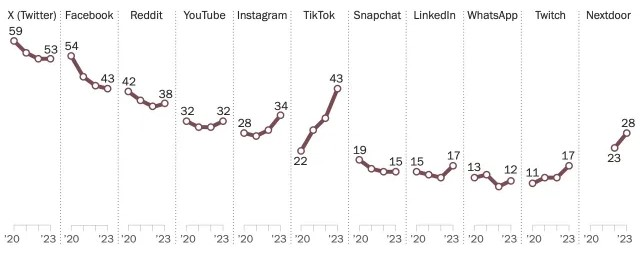
\includegraphics[width=0.80\textwidth]{1/figures/Tendencias_Redes_2023.jpg}
        \caption[Porcentaje de usuarios en base a su consumo de noticias en redes sociales en 2023]{Porcentaje de usuarios en base a su consumo de noticias en redes sociales en 2023. \\ Fuente: \cite{pewresearch_cite}. \textit{Encuesta a adultos de EEUU realizada en 2023}.}
        \label{1:fig}
    \end{center}
\end{figure}

De acuerdo a la \ref{1:fig}, se puede observar que plataformas con tendencia a `Más información en menos tiempo` empiezan a ser las preferidas entre el público, observando el sorprendente aumento de plataformas comoo Instagram y Tiktok. 
Los medios informativos están tomando en cuenta estos cambios y han iniciado a informar en pocos segundos lo más relevante del día mediante videos cortos en sus redes sociales, para llegar a este tipo de público.
Pero el principal desafío diario es cómo seleccionar el contenido que represente los hechos más importantes ocurrido en la actualidad.

Dentro de esta problemática se encuentra la gran cantidad de información audiovisual que se genera cada minuto y la limitada capacidad de realizar análisis para extraer información significativa. 
Este proceso implica enfrentarse a una serie de desafíos técnicos y operativos que requieren soluciones innovadoras y eficientes. En este contexto, las herramientas de Big Data se destacan como una solución crucial. Estas herramientas proporcionan la infraestructura necesaria para manejar, procesar y analizar grandes volúmenes de datos de manera efectiva.

Con el uso de herramientas como PySpark, es posible gestionar datos distribuidos a gran escala, lo que resulta fundamental para el análisis de videos. PySpark permite procesar los datos de video de manera eficiente, extrayendo y analizando frames para identificar eventos clave o patrones significativos. Esta capacidad es esencial dado que los métodos tradicionales de análisis no son suficientes para manejar la escala y complejidad del contenido audiovisual disponible.

En particular, YouTube juega un papel crucial en este análisis. Según Data Reportal en la \ref{2:fig}, en el contexto peruano, YouTube es la segunda página más visitada, con un promedio de 227 millones de visitas mensuales y 11.4 millones de visitantes únicos al mes en 2023. 
YouTube se convierte así en una fuente inagotable de contenido relevante para el análisis de noticias y eventos actuales. La plataforma no solo alberga una vasta biblioteca de videos, sino que también proporciona metadatos valiosos, como descripciones, etiquetas y estadísticas de visualización, que enriquecen el análisis del contenido. 
Aplicar herramientas de big data en YouTube permite automatizar la extracción y el procesamiento de contenido, facilitando la selección de los clips más relevantes que capturan los eventos importantes del día.

\begin{figure}[h]
    \begin{center}
        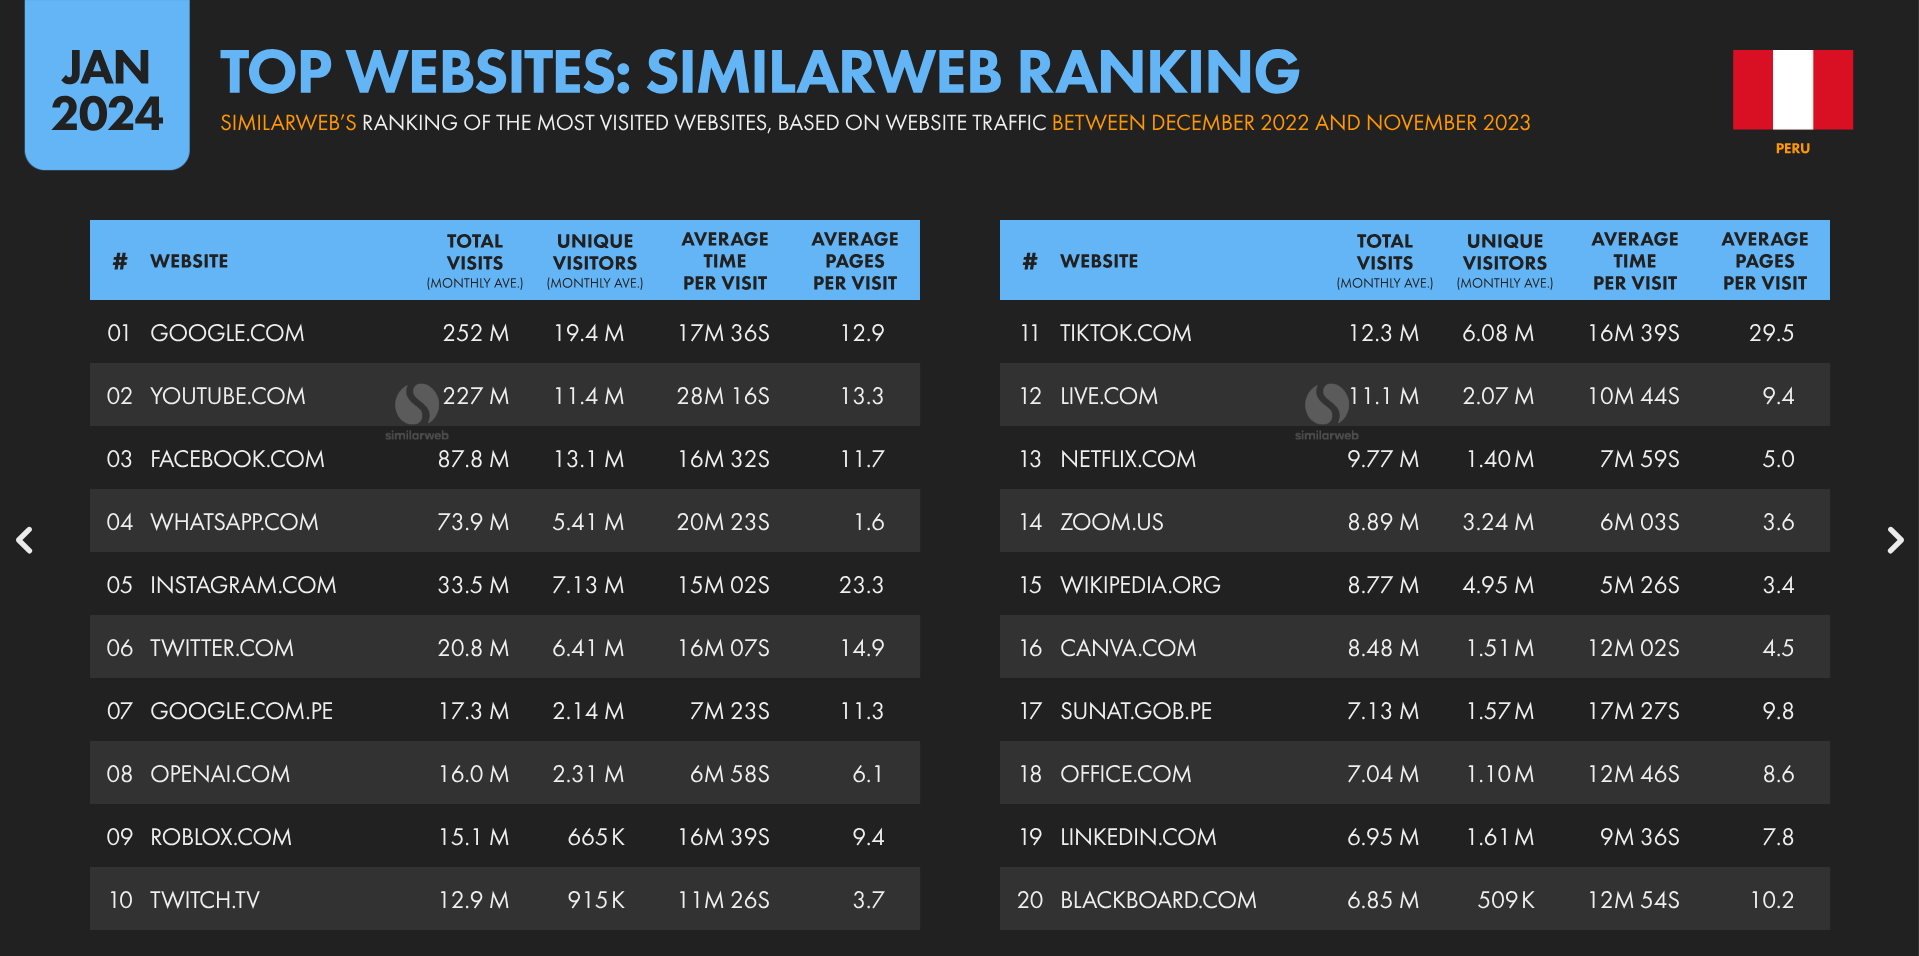
\includegraphics[width=0.80\textwidth]{1/figures/Top_Peru_2023.png}
        \caption[Top webs más visitadas en Perú en 2023]{Top webs más visitadas en Perú en 2023. \\ Fuente: \cite{youtube_peru}. \textit{Basado en el tráfico web de Diciembre de 2022 a Noviembre del 2023}.}
        \label{2:fig}
    \end{center}
\end{figure}

Esta automatización optimiza tanto el tiempo como los recursos necesarios para curar contenido, mejorando la precisión en la selección de información significativa.

La generación de clips informativos a partir de videos largos presenta múltiples beneficios para los medios de comunicación. Primero, facilita la creación de resúmenes concisos y precisos que destacan los puntos clave de las noticias, permitiendo a los usuarios acceder a la información relevante de manera rápida. Este enfoque es crucial en un entorno donde la atención del usuario es limitada y la demanda de contenido digerible es alta.
Esto no solo aumenta el alcance y el impacto de las noticias, sino que también mejora la participación del público y fomenta una mayor interacción con el contenido.

La automatización en la generación de clips también contribuye a la eficiencia operativa de los medios. Al reducir la necesidad de intervención manual en la selección y edición de contenido, los recursos se liberan para enfocarse en otras áreas críticas, como la investigación y el análisis en profundidad. Esto permite a los medios mantenerse competitivos en un entorno en constante cambio y con una demanda creciente de contenido actualizado y relevante.


\subsection{Problema General}
\newcommand{\ProblemaGeneral}{
	¿De qué manera el desarrollo de una herramienta inteligente basada en técnicas de clustering de frames puede facilitar la identificación automática de tendencias a partir de videos de noticieros crear clips de videos representativos?}
\ProblemaGeneral
\subsection{Problemas Espec\'{i}ficos}
\newcommand{\Pbone}{¿Cómo obtener de manera eficiente los videos de noticieros de un día en específico, asegurando que sean representativos de los eventos más importantes del día?}
\newcommand{\Pbtwo}{¿Qué técnicas de preprocesamiento de imágenes y normalización son más efectivas para mejorar la calidad y relevancia de los frames extraídos de los videos?}
\newcommand{\Pbthree}{¿Qué técnicas de extracción de características permiten representar adecuadamente los frames para identificar patrones visuales relevantes?}
\newcommand{\Pbfour}{¿Cuál es el algoritmo de clustering más adecuado para agrupar los frames en base a las similitudes de las características extraídas que posean entre ellas?}
\newcommand{\Pbfive}{¿Cómo generar clips informativos concisos, asegurando que reflejen los eventos clave discutidos en los noticieros?}

\begin{itemize}
	\item \Pbone
	\item \Pbtwo
	\item \Pbthree
	\item \Pbfour
	\item \Pbfive
\end{itemize}

\section{Objetivos de la Investigación}
\subsection{Objetivo General}
\newcommand{\ObjetivoGeneral}{
	Desarrollar una herramienta inteligente que identifique de manera automática tendencias en videos de noticieros mediante el clustering de frames representativos y genere clips de videos que resuman los eventos clave.
}
\ObjetivoGeneral

\subsection{Objetivos Espec\'{i}ficos}
\newcommand{\Objone}{
	Desarrollar un método eficiente para la recolección de videos de noticieros, asegurando que estos reflejen los eventos más importantes del día.
}
\newcommand{\Objtwo}{
	Implementar técnicas de preprocesamiento de imágenes y normalización que mejoren la calidad de los frames extraídos, optimizando su relevancia para el análisis.
}
\newcommand{\Objthree}{
	Desarrollar técnicas de extracción de características que permitan representar adecuadamente los frames, facilitando la identificación de patrones visuales relevantes.
}
\newcommand{\Objtfour}{
	Seleccionar e implementar un algoritmo de clustering que agrupe los frames basándose en la similitud de características, garantizando que los grupos formados representen tendencias claras.
}
\newcommand{\Objtfive}{
	Desarrollar un sistema automatizado para generar clips informativos concisos que resuman los eventos clave identificados en los videos de noticieros.
}


\begin{itemize}
	\item {\Objone}
	\item {\Objtwo}
	\item {\Objthree}
	\item {\Objtfour}
	\item {\Objtfive}
\end{itemize}

\section{Justificación de la Investigación}

\subsection{Teórica}Esta investigación se realiza para determinar cómo el uso de herramientas de Big Data y modelos de aprendizaje automático puede optimizar la selección y generación de clips informativos concisos a partir de contenido audiovisual en YouTube. La teorización se centra en la capacidad de estas herramientas para manejar la sobrecarga de información y mejorar la eficiencia operativa en el proceso de curación de contenido. Este estudio contribuirá al cuerpo de conocimiento en el campo del análisis automatizado de contenido audiovisual, proponiendo un marco teórico para la implementación de tecnologías avanzadas en la industria de los medios de comunicación.
\subsection{Práctica}
Al culminar la investigación, se espera que los medios de comunicación puedan utilizar el sistema automatizado basado en Big Data y aprendizaje automático para seleccionar y generar clips informativos relevantes de manera eficiente. Esto facilitará la creación de resúmenes concisos que destaquen los puntos clave de las noticias, permitiendo a los usuarios acceder a información relevante rápidamente. La implementación práctica de esta solución tecnológica ayudará a los medios a adaptarse a las nuevas tendencias de consumo de contenido, donde la rapidez y concisión son cruciales. Además, mejorará la participación del público y fomentará una mayor interacción con el contenido.
\subsection{Metodológica}. 
El desarrollo del sistema automatizado de análisis de contenido audiovisual utilizando herramientas de Big Data y aprendizaje automático permitirá manejar grandes volúmenes de datos de video de manera eficiente. La metodología incluye el uso de PySpark para la gestión de datos distribuidos y técnicas de procesamiento de imágenes para la extracción de frames significativos. La implementación de algoritmos de clustering ayudará a identificar patrones y eventos relevantes. Esta metodología no solo optimiza el tiempo y los recursos necesarios para curar contenido, sino que también mejora la precisión en la selección de información significativa, ofreciendo una solución tecnológica avanzada para los desafíos actuales en el análisis de contenido audiovisual.
\section{Delimitación del Estudio}

\subsection{Espacial}
El estudio se llevará a cabo en el contexto de plataformas de redes sociales, enfocándose específicamente en YouTube como la principal fuente de contenido audiovisual para el análisis. Se seleccionarán videos de noticias y eventos actuales relevantes para el público peruano, dado que YouTube es una de las páginas más visitadas en Perú, con un alto volumen de visitas mensuales y visitantes únicos. La investigación se centrará en la capacidad de YouTube para proporcionar tanto contenido audiovisual como metadatos valiosos para el análisis.
\subsection{Temporal}
Los datos que se extraerán serán de la primera semana de Agosto del 2024, se realizará la recopilación, procesamiento y análisis. Al ser una herramienta de uso periódico, los resultados se generarán minutos posteriores a la culminación del proceso de recopilación.
\subsection{Conceptual}
La presente investigación se centrará en el desarrollo de un sistema automatizado para la selección y generación de clips informativos a partir de contenido audiovisual utilizando herramientas de Big Data y modelos de aprendizaje automático. El enfoque estará en el análisis de videos de noticias en YouTube, aplicando técnicas de procesamiento de imágenes y algoritmos de clustering para identificar eventos relevantes.
\section{Hipótesis}

\subsection{Hipótesis General}
\newcommand{\HipotesisGeneral}{
	Mediante el uso de técnicas de modelos de aprendizaje automático, se logrará mejorar la identificación de tendencias y la generación de clips informativos representativos de videos de noticieros.
}
\HipotesisGeneral

\HipotesisGeneral
\subsection{Hipótesis Específicas}
\newcommand{\Hone}{
	La recolección automatizada de videos de noticieros de un día específico permitirá capturar de manera eficiente los contenidos más representativos para el análisis de tendencias.
}
\newcommand{\Htwo}{
	El uso de técnicas avanzadas de preprocesamiento y normalización de imágenes mejorará significativamente la calidad de los frames, facilitando su clasificación y análisis posterior.
}
\newcommand{\Hthree}{
	La extracción de características adecuadas de los frames permitirá identificar correctamente patrones visuales que reflejen temas importantes y eventos clave.
}
\newcommand{\Hfour}{
	El uso de un algoritmo de clustering optimizado permitirá agrupar los frames con precisión en función de sus similitudes, identificando adecuadamente las tendencias en los noticieros.
}
\newcommand{\Hfive}{
	La generación automatizada de clips informativos basados en las tendencias identificadas ofrecerá resúmenes concisos y efectivos de los eventos más relevantes del día.
}
\begin{itemize}
	\item \Hone
	\item \Htwo
	\item \Hthree
	\item \Hfour
	\item \Hfive
\end{itemize}

\subsection{Matriz de Consistencia}
A continuación se presenta la matriz de consistencia elaborada para la presente investigación (véase Anexo \ref{1:table}).


\chapter{MARCO TEÓRICO}
\section{Antecedentes de la investigación}
En esta sección se presentarán diversos artículos de investigación o tesis las cuales abordarán diversas técnicas y enfoques que se emplearon para afrontar problemas similares al de esta tesis. Asimismo, a continuación se presenta un cuadro resumen (véase Anexo \ref{A:table}) de lo que se presenta en esta sección.


\subsection{Efficient Video Classification Using Fewer Frames}
\cite{bhardwaj2019efficient}
\subsubsection{Planteamiento del problema}
La necesidad de reducir las operaciones de punto flotante (FLOPs) y la huella de memoria. Aunque los modelos compactos actuales son más ligeros en términos de memoria, todavía requieren un número significativo de FLOPs ya que procesan todos los cuadros de un video. La propuesta de esta investigación es desarrollar modelos de clasificación de videos que procesen menos cuadros, disminuyendo así el número de FLOPs.
\subsubsection{Objetivos}

\begin{itemize}
	\item Desarrollar modelos de clasificación de video que tengan una huella de memoria pequeña (menor a 1 GB) y que sean eficientes 
	\item Crear modelos que procesen menos cuadros de video para reducir el número de FLOPs, manteniendo una alta eficiencia computacional.
	\item Utilizar un modelo maestro computacionalmente intensivo que procesa todos los cuadros para entrenar a un modelo estudiante más eficiente que procesa solo una fracción de los cuadros.
	\item Realizar una evaluación exhaustiva con tres tipos de modelos de clasificación de video: modelos recurrentes, modelos de agrupación y agregación, y modelos de agrupación y agregación eficientes en memoria.
\end{itemize}

\subsubsection {Metodología}
La metodología del documento incluye varias etapas, a partir de la recolección de datos hasta la implementación del modelo. A continuación, se presenta un resumen de la metodología:

\begin{enumerate}
	\item \textbf{Recopilación de datos}: Se utilizó el conjunto de datos YouTube-8M (versión 2017), que contiene 8 millones de videos con múltiples clases asociadas a cada video. Los videos tienen una longitud promedio de 200 segundos.
	\item \textbf{Entrenamiento del profesor y estudiante}:  Se entrena una red neuronal compleja (profesor) que procesa todos los fotogramas de un video para generar una representación detallada del mismo.Se seleccionan solo algunos fotogramas del video (cada j-ésimo fotograma) para ser procesados por la red neuronal del estudiante.e entrena una red neuronal más simple (estudiante) para que genere representaciones similares a las del profesor, utilizando solo los fotogramas seleccionados.
	\item \textbf{Minimización de pérdidas}:Se minimizan las diferencias entre las representaciones del profesor y del estudiante mediante funciones de pérdida específicas, como la pérdida de error cuadrático.
	\item \textbf{Evaluación y Comparación}:Se evalúa el rendimiento del estudiante en términos de precisión y eficiencia computacional, comparándolo con el modelo del profesor y otros métodos base.
\end{enumerate}


\subsubsection{Resultados}

Los resultados obtenidos se presentan en un cuadro comparativo entre los diferentes modelos utilizados en el estudio. Los modelos comparativos 1 y 2 representan otras configuraciones de modelos de aprendizaje profundo probadas por los autores para comparar la efectividad de DeepASL.
\begin{table}[h]
    \centering
    \caption{Resultados de la Clasificación de Videos Utilizando Menos Fotogramas}
    \begin{tabular}{lccccc}
        \hline
        \textbf{Modelo} & \textbf{k} & \textbf{GAP} & \textbf{mAP} & \textbf{FLOPs (Billones)} & \textbf{Tiempo de Evaluación (hrs.)} \\
        \hline
        Teacher-Skyline & N/A  & 0.811 & 0.414 & 5.058 & 13.00 \\
        Uniform-k       & 10   & 0.759 & 0.324 & 0.167 & 7.61  \\
        Uniform-k       & 20   & 0.785 & 0.363 & 0.268 & 8.20  \\
        Uniform-k       & 30   & 0.795 & 0.378 & 0.520 & 9.11  \\
        \hline
    \end{tabular}
    \label{table:video_classification}
    \begin{flushleft}
    \textit{Nota}. GAP = Precision Global Ajustada; mAP = Media de Precisión. FLOPs se refiere a las operaciones de punto flotante.
    \end{flushleft}
\end{table}



\subsection{An improved deep convolutional neural network-based YouTube video classification using textual features}
\cite{raza2024improved}
\subsubsection{Planteamiento del problema}
El artículo aborda el desafío del crecimiento exponencial del contenido de video en plataformas como YouTube, donde se suben más de 30,000 videos por hora, lo que crea la necesidad de categorizar automáticamente este contenido para hacerlo accesible a los usuarios. Las técnicas actuales de clasificación de videos, que se basan en el análisis de texto (como títulos, descripciones y etiquetas), son limitadas en precisión y no han sido suficientemente estudiadas para manejar la vasta cantidad de categorías disponibles. Además, el procesamiento de video e imagen es computacionalmente costoso, lo que impulsa el interés en enfoques basados en texto, que son más eficientes pero subdesarrollados. El artículo sugiere que se requiere un enfoque avanzado de inteligencia artificial que pueda mejorar la categorización de videos utilizando información textual de manera más eficaz y precisa.
\subsubsection{Objetivos}
\begin{itemize}
	\item Realizar un análisis exploratorio de datos de YouTube para obtener información sobre los videos y sus categorías, identificando patrones y tendencias clave.
	\item Desarrollar un modelo mejorado de red neuronal convolucional profunda (DCNN) que permita categorizar videos de YouTube con alta precisión y eficiencia.
	\item Comparar el rendimiento del modelo DCNN con otros enfoques de aprendizaje profundo, como redes neuronales recurrentes (RNN) y unidades de memoria a largo plazo (GRU), así como con modelos de aprendizaje automático tradicionales, como la regresión logística, máquinas de soporte vectorial (SVM), árboles de decisión y bosques aleatorios.
\end{itemize}

\subsubsection {Fundamento Teórico}
Dado que el procesamiento de imágenes y videos es computacionalmente costoso, el estudio explora el uso de características textuales (títulos, descripciones y etiquetas) para clasificar los videos de manera más eficiente. En este contexto, se propone un modelo de red neuronal convolucional profunda (DCNN) como enfoque principal para la categorización de videos, destacando su capacidad para manejar grandes volúmenes de datos con alta precisión. El estudio compara el desempeño del modelo DCNN con otros modelos de aprendizaje profundo, como las redes neuronales recurrentes (RNN) y las unidades de memoria a largo plazo (GRU), demostrando que el DCNN supera a estos enfoques en términos de precisión y eficiencia en la clasificación de videos.
\subsubsection {Metodología: }
	\begin{enumerate}
		\item \textbf{Adquisición de datos}: 
		\begin{itemize}
			\item Este conjunto de datos contiene 20,000 videos categorizados en 9 temas como aventura, arte y música, ciencia, deportes, entre otros.
		\end{itemize}
		
		\item \textbf{Preprocesamiento textual}:
		\begin{itemize}
			\item Limpieza de ruido en los textos de los títulos y descripciones de los videos. Se transforman los textos a minúsculas, se eliminan números, puntuaciones y espacios en blanco adicionales. El proceso incluye tokenización, eliminación de tokens no alfabéticos y palabras vacías, finalizando con la lematización para convertir las palabras a sus formas raíz.
			\item Análisis estadístico tanto a nivel observacional como de corpus. Se evalúan medidas como el tamaño promedio del vocabulario y la riqueza léxica de las descripciones.
			\item  El conjunto de datos se divide en un 80\% para entrenamiento y un 20\% para pruebas, con el objetivo de entrenar
			\end{itemize}
		
		\item \textbf{Entrenamiento del modelo}:
		\begin{itemize}
			\item Se Se implementan redes neuronales recurrentes (RNN) y unidades de memoria controlada (GRU) para procesar secuencias textuales. Se explica cómo estas redes manejan datos secuenciales mediante conexiones entre capas y se optimizan a través de capas de dropout y activación.
		\end{itemize}
		
		\item \textbf{Categorización de los videos}:
		\begin{itemize}
			\item Se desarrolla una red neuronal convolucional profunda (DCNN) para la clasificación de videos. El modelo utiliza capas de convolución, agrupamiento y capas densas, optimizando sus parámetros y estructura para obtener un alto rendimiento en la categorización.
		\end{itemize}
	\end{enumerate}
	\begin{figure}[h]
		\centering
		\includegraphics[width=0.5\textwidth]{2/figures/Metodología.png}
		\caption{Metodología}
		\label{fig:etiqueta_de_la_figura}
	\end{figure}

	\subsubsection{Resultados: }
	Los resultados del artículo se presentan en la siguiente tabla:
	
	\begin{table}[h]
		\centering
		\caption{Resultados experimentales de los modelos}
		\begin{tabular}{lccc}
			\hline
			\textbf{Modelo} & \textbf{Precisión (\%)} & \textbf{AUC (\%)} & \textbf{Puntuación F1} \\
			\hline
			DCNN & 96 & 99 & 0.95 \\
			RNN  & 92 & 97 & 0.91 \\
			GRU  & 94 & 98 & 0.93 \\
			\hline
		\end{tabular}
		\label{table:model_results}
	\end{table}







\subsection{TV News Database Indexing System with Video Structure Analysis, Representative Images Extractions and OCR for News Titles}
\cite{rozsa2022tv}

\subsubsection{Planteamiento del Problema}
El problema abordado en este trabajo es la falta de sistemas eficientes para la indexación y recuperación de contenido en archivos de video, particularmente en los programas de noticias televisivas. Muchas cadenas de televisión acumulan grandes cantidades de material de video, tanto en formatos analógicos como digitales, que no están organizados en sistemas de gestión de contenido que permitan búsquedas rápidas y reutilización del material. Esto dificulta la recuperación eficiente de información para la creación de nuevos contenidos o la supervisión del cumplimiento de las transmisiones.
\subsubsection{Objetivos}
\begin{itemize}
	\item Desarrollar un sistema semiautomático para analizar la estructura temporal de los programas de noticias televisivas.
	\item Implementar métodos de segmentación de video y extracción de imágenes representativas para mejorar la indexación de contenido.
	\item Aplicar reconocimiento óptico de caracteres (OCR) para extraer títulos de noticias y facilitar su búsqueda y recuperación.
	\item Probar el sistema propuesto en diferentes programas de noticias y evaluar su eficiencia en comparación con otros métodos.
\end{itemize}
\subsubsection{Fundamento Teórico}

El trabajo se basa en la necesidad de sistemas de gestión de contenido multimedia que puedan indexar y categorizar de manera eficiente los programas de televisión, especialmente las noticias. Se hace uso de tecnologías como la segmentación de video, la extracción de fotogramas clave y el OCR, que permite reconocer texto en imágenes. La segmentación del video se realiza analizando secuencias de fotogramas y detectando cambios significativos mediante histogramas de color y nivel de gris. Posteriormente, se extraen imágenes representativas para facilitar la navegación y búsqueda dentro de los archivos. La integración del OCR permite reconocer los títulos de las noticias, lo que facilita su búsqueda en la base de datos.

\subsubsection {Metodología }
\begin{enumerate}
	\item \textbf{Segmentación de video}:
	\begin{itemize}
		\item Se identifican puntos de inicio y fin de las tomas y se extraen imágenes representativas para cada toma. Para ello, se calcula la diferencia entre los histogramas de color de fotogramas sucesivos, utilizando métricas como la distancia de Bhattacharyya.
	\end{itemize}
	
	\item \textbf{Extracción de imágenes representativas}:
	\begin{itemize}
		\item se seleccionan imágenes representativas para cada toma con el fin de facilitar la búsqueda. Este proceso se realiza adaptando los umbrales de discriminación dependiendo de la complejidad del material.
	\end{itemize}
	
	\item \textbf{Reconocimiento óptico de caracteres (OCR)}:
	\begin{itemize}
		\item Se extrae títulos de noticias a partir de áreas predefinidas en la imagen. Se aplica preprocesamiento a las imágenes (conversión a escala de grises, umbralización) para mejorar la precisión de la extracción de texto.
	\end{itemize}
	
	\item \textbf{Evaluación del sistema}:
	\begin{itemize}
		\item  El sistema fue probado en programas de noticias de varias cadenas de televisión de Rumania, midiendo el tiempo de análisis y el número de imágenes útiles extraídas para la indexación en la base de datos.
	\end{itemize}
\end{enumerate}
	
\subsubsection{Resultados: }

\begin{table}[h]
    \centering
    \caption{Resultados experimentales de la segmentación de video en noticias televisivas}
    \begin{tabular}{lcc}
        \hline
        \textbf{Canal de TV} & \textbf{Duración del programa (min)} & \textbf{Imágenes extraídas} \\
        \hline
        ProTV, TVR1, Kanal D, Prima TV, Intermedia & 40--45 & 800--900 \\
        \hline
    \end{tabular}
    \label{tab:segmentacion}
    \begin{flushleft}
    \textit{Nota}. Los resultados muestran la duración promedio de los programas de noticias y el número de imágenes extraídas por programa en varios canales de televisión.
    \end{flushleft}
\end{table}


\noindent \textbf{Descripción de los resultados:} Los experimentos se realizaron con programas de noticias de 40 a 45 minutos de duración de cinco canales de televisión distintos. El sistema propuesto para la segmentación de video extrajo entre 800 y 900 imágenes representativas por programa, que son utilizadas para la indexación en una base de datos de noticias televisivas. La cantidad de imágenes extraídas varía según el contenido y el estilo de producción de cada canal, pero en todos los casos se logró una segmentación precisa del contenido, facilitando la búsqueda y recuperación de material archivado.


\subsection{Shear Detection and Key Frame Extraction of Sports Video Based on Machine Learning}
\cite{wang2023shear}
\subsubsection{Planteamiento del Problema}

El trabajo aborda el problema del crecimiento exponencial de los datos de video, lo que ha generado la necesidad de herramientas eficientes para procesar, analizar y recuperar el contenido. En particular, los videos deportivos presentan desafíos debido a la diversidad de tomas y cambios rápidos en los ángulos de cámara, lo que dificulta la detección de cortes y la extracción de fotogramas clave que representen de manera precisa el contenido de las escenas.

\subsubsection{Objetivos}
\begin{itemize}
	\item Proponer un método basado en el análisis del movimiento para detectar los cortes de escena en videos deportivos.
	\item Desarrollar un algoritmo que permita la extracción automática de fotogramas clave representativos de las escenas deportivas.
	\item Reducir el volumen de datos en los índices de video mediante la selección de fotogramas clave sin comprometer la representación visual.
	\item Crear una plataforma de navegación de videos basada en fotogramas clave que facilite la búsqueda y recuperación del contenido deportivo.
\end{itemize}

\subsubsection{Fundamento Teórico}
El trabajo se fundamenta en la teoría del aprendizaje automático (ML) y el procesamiento de video. El análisis de video basado en el contenido (Content-Based Video Analysis) permite una mejor comprensión de los datos visuales mediante técnicas de visión por computadora y procesamiento de imágenes. La detección de cortes y la extracción de fotogramas clave son aspectos esenciales para la organización y recuperación de videos. Los modelos de ML, como el SVM, se utilizan para clasificar patrones en los datos visuales, mientras que los algoritmos de estimación de movimiento, basados en el bloque de coincidencia, permiten identificar transiciones entre fotogramas y escenas.
\subsubsection{Metodología}

\begin{enumerate}
	\item \textbf{Estimación del movimiento basado en bloques}:
	\begin{itemize}
		\item El algoritmo divide el video en bloques de píxeles y calcula la similitud de los bloques entre fotogramas consecutivos para identificar cambios significativos de movimiento. Esto permite detectar los cortes de escena basados en el movimiento.
	\end{itemize}
	
	\item \textbf{Detección de cortes mediante SVM}:
	\begin{itemize}
		\item El modelo de máquina de soporte vectorial (SVM) clasifica las transiciones entre fotogramas como cortes graduales o no graduales, utilizando características extraídas de los vectores de movimiento.
	\end{itemize}
	
	\item \textbf{Extracción de fotogramas clave}:
	\begin{itemize}
		\item Se utiliza un modelo de atención del usuario para determinar la relevancia de cada fotograma dentro de una escena. Los fotogramas con mayor valor de atención se seleccionan como representativos, permitiendo así una navegación más eficiente del video.
	\end{itemize}
	
	\item \textbf{Evaluación experimental}:
	\begin{itemize}
		\item El sistema fue probado en videos deportivos, midiendo su eficiencia en la detección de cortes y la capacidad de reducir el volumen de datos en los índices de video. La plataforma generada permite navegar a través de los fotogramas clave para visualizar resúmenes del contenido.
	\end{itemize}
\end{enumerate}

\subsubsection{Resultados}

El sistema de detección de cortes y extracción de fotogramas clave propuesto demuestra ser eficiente y preciso. El uso del modelo basado en aprendizaje automático ha permitido una mejor detección de transiciones graduales y no graduales en videos deportivos, además de la extracción precisa de fotogramas clave. Este sistema puede aplicarse a múltiples tipos de videos sin necesidad de entrenamientos específicos para cada tipo, lo que mejora la eficiencia en el análisis y la recuperación de videos en entornos de alto volumen de datos.


\subsection{Research on Key Frame Extraction of Digital Image Based on Unsupervised Clustering Algorithm}
\cite{wang2023keyframe}
\subsubsection{Planteamiento del Problema}
Con el crecimiento exponencial de la información multimedia, el procesamiento eficiente de grandes volúmenes de datos de video se ha convertido en un desafío clave. Los métodos tradicionales para la extracción de fotogramas clave son ineficientes para manejar videos a gran escala y presentan limitaciones en cuanto a la precisión y velocidad de procesamiento. Esto genera una necesidad urgente de desarrollar técnicas más avanzadas que permitan extraer automáticamente los fotogramas más representativos de un video, facilitando su análisis y almacenamiento.
\subsubsection{Objetivos}
\begin{itemize}
	\item Proponer un método de extracción de fotogramas clave basado en un algoritmo de clustering no supervisado.
	\item Mejorar la precisión en la detección de fotogramas clave en videos digitales mediante el uso de algoritmos de aprendizaje automático.
	\item Reducir el tiempo de procesamiento en la extracción de fotogramas clave, optimizando la eficiencia del sistema.
	\item Validar la efectividad del algoritmo propuesto mediante simulaciones y comparaciones con modelos tradicionales de extracción de fotogramas clave.
\end{itemize}
\subsubsection{Fundamento Teórico}
El artículo se basa en el uso de algoritmos de clustering no supervisados para clasificar fotogramas de video según su similitud, permitiendo identificar aquellos más representativos de una escena. La extracción de fotogramas clave es crucial para la recuperación y análisis de contenido en videos, ya que permite generar resúmenes concisos. A diferencia de los métodos tradicionales, que dependen de intervalos de tiempo o reglas de calidad de imagen, el clustering no supervisado se enfoca en descubrir automáticamente patrones de similitud en los datos, lo que mejora la precisión de la extracción de fotogramas. La combinación con redes neuronales RBF permite modelar y ajustar mejor las trayectorias y patrones de movimiento en los videos.
\subsubsection{Metodología}

\begin{enumerate}
	\item \textbf{Extracción de características basadas en segmentación}:
	\begin{itemize}
		\item El video se segmenta en bloques de imagen, de los cuales se extraen características como el histograma de color, la textura y la forma. Estas características se agrupan en un vector para cada bloque de imagen, lo que permite realizar una comparación entre fotogramas.
	\end{itemize}
	
	\item \textbf{Cálculo de distancias de similitud}:
	\begin{itemize}
		\item Se utiliza la distancia Euclidiana para medir la similitud entre fotogramas, normalizando previamente los vectores de características. Esto permite identificar fotogramas que contienen información novedosa y los clasifica como candidatos a fotogramas clave.
	\end{itemize}
	
	\item \textbf{Algoritmo de clustering no supervisado}:
	\begin{itemize}
		\item El algoritmo realiza un análisis de movimiento y características de contenido entre los fotogramas. Agrupa fotogramas similares en clusters y selecciona aquellos que mejor representan el video. El proceso se optimiza mediante el uso de redes neuronales RBF, que ajustan las trayectorias de movimiento y optimizan la selección de fotogramas clave.
	
	\item \textbf{Evaluación experimental}:
	\begin{itemize}
		\item Se realizaron simulaciones con diferentes tipos de videos para comparar el rendimiento del algoritmo propuesto con modelos tradicionales. Los resultados mostraron una mayor precisión en la extracción de fotogramas clave y una reducción en el tiempo de procesamiento.
	\end{itemize}
\end{enumerate}


\subsubsection{Resultados}

\begin{table}[h]
    \centering
    \caption{Resultados de la extracción de fotogramas clave y detección de cortes en videos}
    \begin{tabular}{lcc}
        \hline
        \textbf{Método} & \textbf{Precisión (\%)} & \textbf{Tiempo de procesamiento (segundos)} \\
        \hline
        Clustering no supervisado & 95.45 & 120 \\
        Modelo de mezcla gaussiana & 89.32 & 150 \\
        Algoritmo de movimiento & 92.11 & 135 \\
        \hline
    \end{tabular}
\end{table}


\noindent \textbf{Resumen de los resultados:} 
El algoritmo de clustering no supervisado propuesto demostró ser más preciso y eficiente que los métodos comparados, lo que lo convierte en una solución efectiva para la extracción de fotogramas clave en grandes volúmenes de datos de video. Esto sugiere que este enfoque tiene un gran potencial para aplicaciones en análisis de video en tiempo real y en escenarios donde se requiere procesamiento rápido de datos

\subsection{NewsVideo Summarization Combining SURF and Color Histogram Features}
\cite{liang2021news}
\subsubsection{Planteamiento del Problema}
El volumen de videos noticiosos ha crecido exponencialmente, lo que hace necesario contar con métodos eficientes para resumirlos y facilitar su consumo. Los métodos actuales de resumen de video no siempre capturan la complejidad de los videos debido a la variabilidad en las transiciones entre escenas. Además, muchos de los enfoques existentes fallan en la detección precisa de los límites entre escenas debido a los cambios en la complejidad visual, lo que resulta en resúmenes de video poco representativos.
\subsubsection{Objetivos}
\begin{itemize}
	\item Proponer un método novedoso para la detección de límites de escenas basado en características SURF.
	\item Desarrollar un algoritmo mejorado de clustering que no requiera predefinir el número de clusters y pueda adaptarse a la complejidad visual de las escenas.
	\item Reducir la redundancia en los marcos clave seleccionados para representar mejor el contenido del video noticioso.
	\item Validar la eficacia del método propuesto mediante experimentos en datasets públicos y autoconstruidos.
\end{itemize}
\subsubsection{Fundamento Teórico}
El artículo se basa en el uso de características locales, como las características SURF (Speeded Up Robust Features), que son invariantes ante rotaciones, cambios de escala y variaciones de iluminación. Estas características permiten una mayor precisión en la detección de límites entre escenas, en comparación con métodos que dependen de características globales como los histogramas de color. 

El algoritmo SURF se utiliza para identificar puntos clave en los fotogramas, lo que permite comparar la similitud entre ellos. Además, el uso de un algoritmo de clustering mejorado basado en histogramas HSV permite extraer los marcos clave más representativos de cada escena.
\subsubsection {Metodología }
\begin{enumerate}
	\item \textbf{Preprocesamiento de datos}:
	\begin{itemize}
		\item  Se eliminan elementos estáticos, como logotipos o subtítulos rodantes, que pueden interferir con la detección de límites de escena.
	\end{itemize}
	
	\item \textbf{Extraer características}:
	\begin{itemize}
		\item  Se extraen puntos de interés locales y se comparan entre fotogramas adyacentes utilizando el algoritmo FLANN para acelerar el proceso.
	\end{itemize}
	
	\item \textbf{Similitud entre fotogramas}:
	\begin{itemize}
		\item A partir de las coincidencias entre características SURF, se genera una curva de similitud que permite identificar transiciones abruptas y graduales entre escenas.
	\end{itemize}
	
	\item \textbf{Clustering basado en histogramas}:
	\begin{itemize}
		\item Se agrupan los fotogramas de cada escena según sus histogramas de color. El algoritmo ajusta dinámicamente el número de clusters para reflejar la complejidad visual de la escena.
	\end{itemize}
	
	\item \textbf{Selección de marcos clave}:
	\begin{itemize}
		\item  Se elige el fotograma más cercano al centro de cada cluster como representante clave de esa escena, garantizando que los marcos seleccionados representen fielmente el contenido del video.
	\end{itemize}
\end{enumerate}
	
\subsubsection{Resultados:}

\begin{table}[h]
    \centering
    \caption{Resultados de la detección de límites de escenas por tipo de video}
    \begin{tabular}{lcc}
        \hline
        \textbf{Tipo de Video} & \textbf{Recall (\%)} & \textbf{Precisión (\%)} \\
        \hline
        News in 30 Minutes     & 96.57 & 97.24 \\
        CCTV News              & 100.00 & 94.29 \\
        Sports Express         & 96.05 & 85.88 \\
        \hline
        \textbf{Total}         & 97.22 & 93.33 \\
        \hline
    \end{tabular}
\end{table}

\begin{table}[h]
    \centering
    \caption{Comparación de métodos de detección de límites de escenas}
    \begin{tabular}{lcc}
        \hline
        \textbf{Método} & \textbf{Recall (\%)} & \textbf{Precisión (\%)} \\
        \hline
        Ours             & 97.22 & 93.33 \\
        Feng        & 86.48 & 93.20 \\
        Wang       & 90.41 & 94.28 \\
        Rachida  & 96.49 & 95.87 \\
        TransNetV2   & 92.68 & 98.52 \\
        \hline
    \end{tabular}
    \begin{flushleft}
    \textit{Nota}. Comparación de los resultados de distintos métodos para la detección de límites de escenas.
    \end{flushleft}
\end{table}


\begin{table}[h]
    \centering
    \caption{Comparación de métodos en el dataset TVSum50}
    \begin{tabular}{lcc}
        \hline
        \textbf{Método} & \textbf{Recall (\%)} & \textbf{Precisión (\%)} \\
        \hline
        Ours             & 95.93 & 87.91 \\
        TransNetV2   & 92.56 & 92.02 \\
        \hline
    \end{tabular}
\end{table}

\section{Bases Teóricas}
\subsection{Preprocesamiento de imágenes}\label{sec:preprocesamiento_imagenes}
Antes de aplicar el clustering a imágenes, es fundamental realizar un preprocesamiento que generalmente incluye:

\begin{itemize}
    \item \textbf{Extracción de características}: Las imágenes se transforman en vectores de características que describen aspectos relevantes de su contenido. Algunos métodos comunes incluyen:
        \begin{itemize}
            \item El \textit{Histogram of Oriented Gradients} (HOG) es un descriptor utilizado ampliamente en el procesamiento de imágenes y la visión por computadora para la detección de objetos. Introducido por Dalal y Triggs, HOG permite capturar las características locales de una imagen basándose en la distribución de los gradientes de intensidad. Este método es especialmente útil para delinear bordes y contornos en imágenes.

            Para calcular el HOG, una imagen se divide en pequeñas celdas (o patches), y dentro de cada celda se computa un histograma de la orientación de los gradientes. La magnitud y dirección del gradiente en cada píxel se obtienen aplicando filtros de derivadas en las direcciones horizontal y vertical, según las siguientes fórmulas:
            
            \[G_x = I(x+1, y) - I(x-1, y)
            \]
            \[G_y = I(x, y+1) - I(x, y-1)
            \]

            donde \(G_x\) y \(G_y\) representan los gradientes en las direcciones horizontal y vertical, respectivamente.

            La magnitud del gradiente \(M(x, y)\) y su orientación \(\theta(x, y)\) se calculan como:

            \[M(x, y) = \sqrt{G_x^2 + G_y^2}
            \]
            \[\theta(x, y) = \text{arctan2}(G_y, G_x)
            \]

            Posteriormente, se construye un histograma de orientaciones para cada celda, el cual se normaliza para mejorar la resistencia a los cambios de iluminación y contraste. Los histogramas de todas las celdas se concatenan para formar el descriptor final.
            
            \begin{figure}[H]
                \centering
                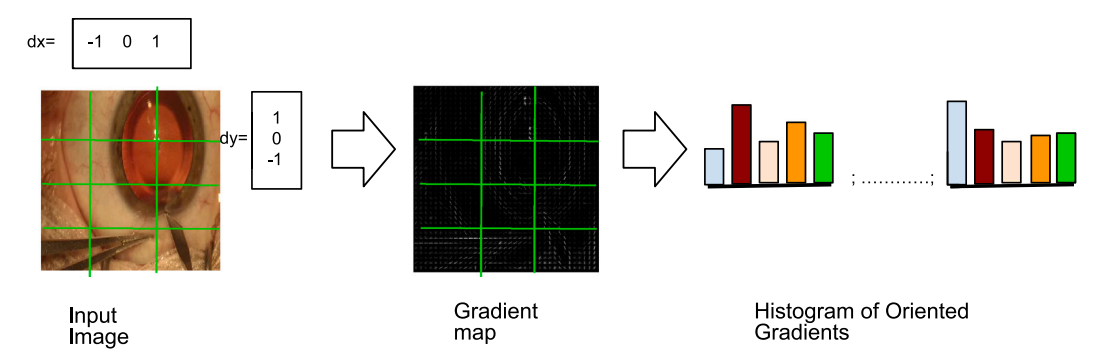
\includegraphics[width=0.80\textwidth]{2/figures/HOG.png}
                \caption{Proceso de Histogram of Oriented Gradients (HOG). Fuente:\cite {bhattarai2023hog}.}

                \label{1:fig}
            \end{figure}
            

        \end{itemize} 
\end{itemize}


\subsection{Deep Learning}
El Deep Learning ha transformado el campo del procesamiento de imágenes al permitir la automatización de tareas complejas como la clasificación, detección de objetos y segmentación de imágenes. Las redes neuronales profundas, particularmente las redes neuronales convolucionales (CNNs), son la arquitectura principal utilizada para el análisis de imágenes debido a su capacidad para capturar características espaciales jerárquicas en los datos visuales.


\begin{figure}[H]
    \centering
    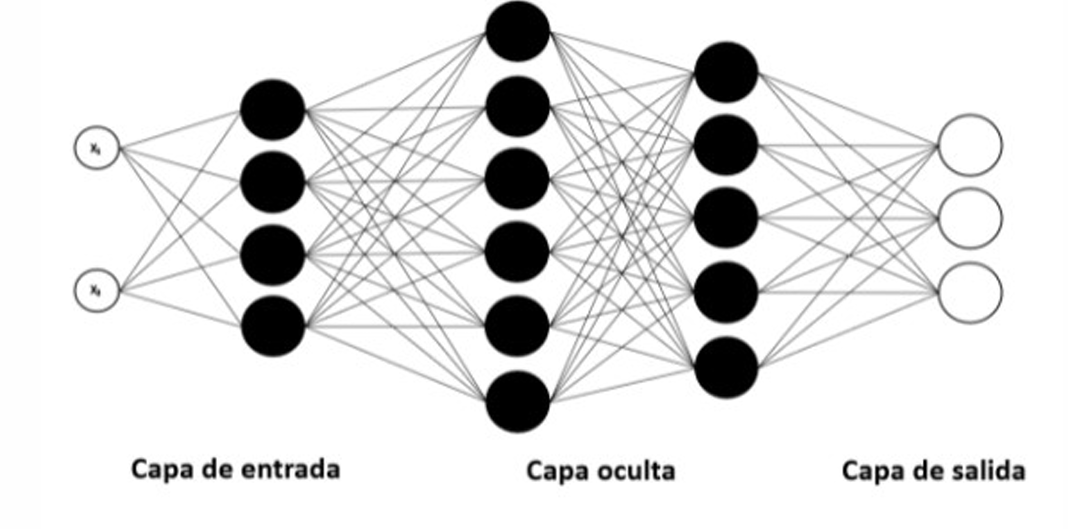
\includegraphics[width=0.60\textwidth]{2/figures/Redes neuronales.png}
    \caption{Estructura de una red neuronal. Fuente: Elaboración propia.}

\end{figure}

\subsubsection{Redes Neuronales Convolucionales (CNNs)}
Las Redes Neuronales Convolucionales (CNNs) constituyen una arquitectura clave dentro del Deep Learning, ampliamente reconocida por su eficacia en el análisis de imágenes. Su principal fortaleza radica en su capacidad para aprender representaciones jerárquicas de los datos visuales, lo que les permite captar patrones espaciales complejos. Las CNNs logran esta tarea mediante el uso de múltiples capas especializadas que procesan la información de manera progresiva.

Cada una de estas capas realiza la extracción automática de características relevantes de las imágenes, optimizando su capacidad de detección y clasificación durante el proceso de entrenamiento. Esta estructura en capas permite que las CNNs identifiquen desde bordes simples hasta patrones más abstractos, a medida que la información fluye desde las capas iniciales hacia las más profundas del modelo.

\begin{itemize} 
    \item 
    \textbf{Capa convolucional}: Esta capa aplica filtros (o kernels) sobre la imagen para extraer características locales como bordes, texturas y patrones. A medida que cada filtro se desplaza sobre la imagen, se genera un mapa de características que destaca las particularidades locales. Para una imagen de entrada \(X\), el resultado de aplicar un filtro \(K\) es un mapa de características \(F\) dado por:

    \[
    F(i,j) = \sum_m \sum_n X(i+m,j+n) \cdot K(m,n),
    \]

    donde \(m\) y \(n\) son los índices de los elementos del filtro \(K\), y \(i, j\) son los índices de los píxeles en la imagen.

    \begin{figure}[H]
        \centering
        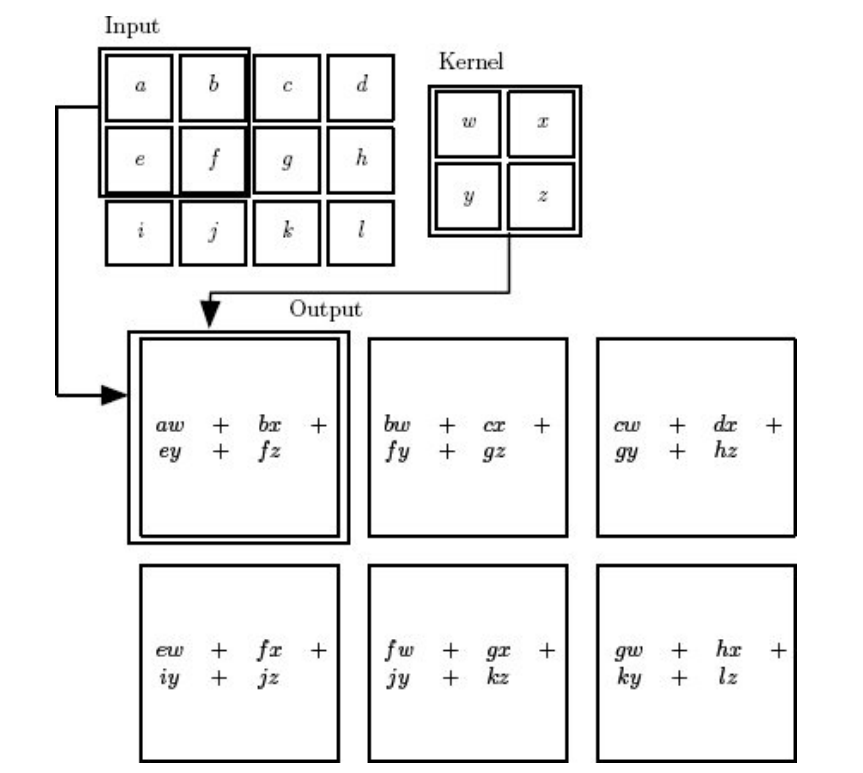
\includegraphics[width=0.40\textwidth]{2/figures/Convolucion.png}
        \caption{Proceso de convolución. Fuente: \cite{Goodfellow-et-al-2016}. \textit{Recuperado de Deep Learning}.}
        \label{fig:convolucion}
    \end{figure}
    

    \item \textbf{Capa de pooling}: Reduce la dimensionalidad de las características extraídas al resumir pequeñas regiones de las imágenes (por ejemplo, mediante el \textit{max-pooling}, que selecciona el valor máximo en cada región). Esto ayuda a reducir el número de parámetros y a controlar el sobreajuste.
\end{itemize}

\subsubsection{ResNet50}

La \textbf{ResNet50} es una arquitectura de red neuronal profunda que pertenece a la familia de las Redes Residuales (ResNet), introducida por He et al. en 2015. ResNet50 destaca por su capacidad para entrenar redes profundas sin enfrentar los problemas de degradación que afectan a las redes convolucionales tradicionales al aumentar en capas. Esto se logra mediante la incorporación de \textit{bloques residuales}, los cuales permiten una mejor propagación del gradiente a lo largo de las capas.

\paragraph{Arquitectura y Estructura de ResNet50}

ResNet50 está compuesta por 50 capas que incluyen convoluciones, \textit{pooling}, y capas totalmente conectadas. La clave de su arquitectura son los \textit{bloques residuales}, en los que la salida de una capa se suma directamente a la salida de una capa posterior, permitiendo que los datos "salten" una o más capas. Esta operación de "salto" ayuda a conservar la información y a mitigar la pérdida del gradiente, un problema común en redes profundas. La estructura de ResNet50 puede dividirse en:
\begin{itemize}
    \item \textbf{Bloques residuales}: Cada bloque consiste en una serie de capas convolucionales, seguidas de una conexión residual que permite sumar la entrada del bloque a la salida de una capa más profunda, facilitando el flujo de información.
    \item \textbf{Capas convolucionales y pooling}: La red comienza con una capa convolucional inicial y una operación de pooling, seguidas de los bloques residuales. Al final de la red, se realiza un \textit{global average pooling} para reducir la dimensionalidad antes de la capa totalmente conectada.
\end{itemize}

\paragraph{Funcionamiento de los bloques residuales}
Los bloques residuales son el componente esencial que diferencia a ResNet50 de otras arquitecturas. En cada bloque, una entrada \( x \) se combina con la salida de una convolución \( F(x) \) mediante una suma: 
\[
y = F(x) + x,
\]
donde \( F(x) \) es la salida de las capas convolucionales del bloque. Esta suma permite que el bloque aprenda la función de residuo en lugar de una transformación completa, lo que facilita el entrenamiento y previene el desvanecimiento del gradiente.

\paragraph{Ventajas de ResNet50}
ResNet50 es ampliamente utilizada como extractor de características en tareas de visión por computadora debido a su capacidad para aprender y representar características visuales complejas. Sus principales ventajas como extractor de características incluyen:

\begin{itemize}
    \item \textbf{Profundidad eficaz}: La arquitectura profunda de ResNet50, soportada por bloques residuales, permite extraer características de alta calidad y precisión sin sufrir degradación de rendimiento, lo que resulta en descriptores visuales detallados y robustos.
    \item \textbf{Capacidad de transferencia de aprendizaje}: Al estar preentrenada en grandes conjuntos de datos como ImageNet, ResNet50 ofrece una base de características generalizables, permitiendo su uso en diversas aplicaciones de extracción de características sin necesidad de entrenar el modelo desde cero.
    \item \textbf{Optimización computacional}: La eficiencia en el flujo de gradientes gracias a los bloques residuales mejora la velocidad de extracción y permite el uso de ResNet50 en múltiples plataformas, facilitando un procesamiento eficiente incluso en sistemas con limitaciones de hardware.
\end{itemize}

\begin{figure}[H]
	\centering
	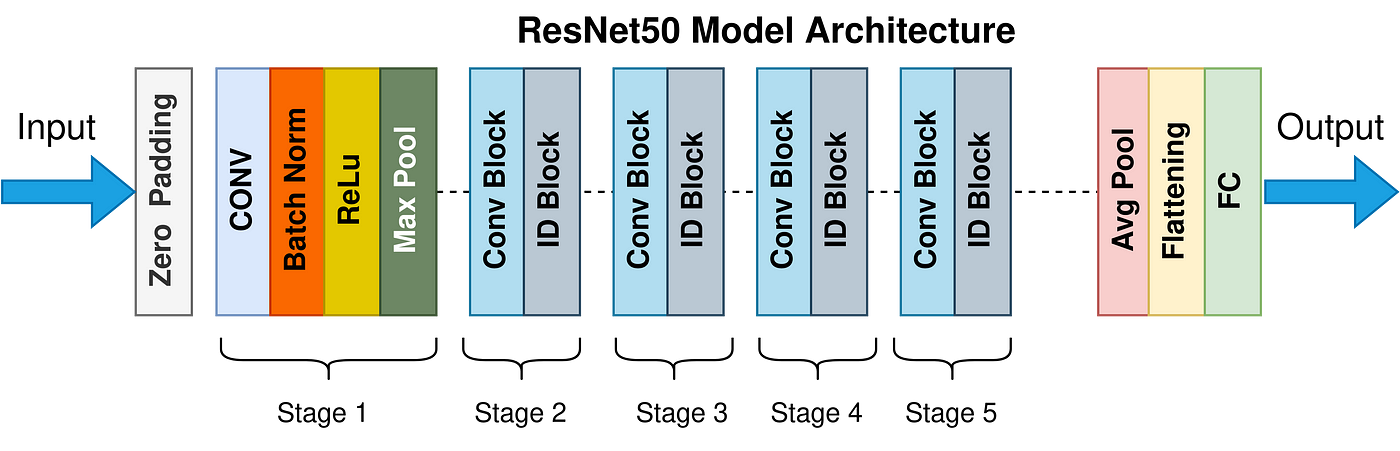
\includegraphics[width=0.80\textwidth]{2/figures/ResNet.png}
	\caption{Arquitectura de ResNet50. Fuente:\cite {Mukherjee2022}.}

	\label{1:fig}
\end{figure}

\subsection{Análisis de Componentes Principales (PCA)}

El \textbf{Análisis de componentes principales} (PCA, por sus siglas en inglés) es una técnica estadística utilizada para la \textit{reducción de dimensionalidad} en conjuntos de datos de alta dimensión. PCA transforma los datos en un espacio de menor dimensión mientras conserva la mayor variabilidad posible, lo cual es útil en el preprocesamiento de datos para reducir la redundancia y simplificar el análisis.

\subsubsection{Funcionamiento de PCA}

El proceso de PCA se basa en los siguientes pasos:

\begin{enumerate}
    \item \textbf{Centramiento de los datos}: 
    Dado un conjunto de datos con \(n\) muestras y \(d\) características, se calcula la media de cada característica y se centra cada variable restando su media. Esto garantiza que el nuevo conjunto de datos tenga una media de cero, simplificando los cálculos subsiguientes. Si \(\mathbf{X}\) representa la matriz de datos original, donde cada columna es una característica, la matriz centrada \(\mathbf{X_c}\) se obtiene restando la media:
    
    \[
    \mathbf{X_c} = \mathbf{X} - \text{mean}(\mathbf{X})
    \]

    \item \textbf{Cálculo de la matriz de covarianza}: 
    La matriz de covarianza \(\mathbf{C}\) representa cómo cada par de variables varía conjuntamente, permitiendo identificar relaciones entre las características originales. La matriz de covarianza se calcula como:

    \[
    \mathbf{C} = \frac{1}{n-1} \mathbf{X_c}^T \mathbf{X_c}
    \]

    donde \(n\) es el número de muestras en el conjunto de datos. Esta matriz es de tamaño \(d \times d\), donde \(d\) es el número de características.

    \item \textbf{Descomposición de la matriz de covarianza en valores y vectores propios}: 
    La descomposición de la matriz de covarianza permite encontrar los \textit{componentes principales}. Se calculan los \textit{vectores propios} y \textit{valores propios} de la matriz de covarianza \(\mathbf{C}\):

    \[
    \mathbf{C} \mathbf{v}_i = \lambda_i \mathbf{v}_i
    \]

    donde \(\mathbf{v}_i\) es el vector propio (o componente principal) y \(\lambda_i\) es su valor propio correspondiente, que representa la varianza explicada por ese componente. Los componentes se ordenan en función de la magnitud de \(\lambda_i\), de mayor a menor, ya que los valores propios más altos representan mayor variabilidad en los datos.

    \item \textbf{Selección de componentes principales}: 
    A menudo, se seleccionan solo los primeros \(k\) componentes principales que explican la mayor parte de la varianza de los datos. La cantidad de varianza explicada por cada componente principal se calcula como:

    \[
    \text{Varianza Explicada} = \frac{\lambda_i}{\sum_{j=1}^{d} \lambda_j}
    \]

    y se suele visualizar en un gráfico de varianza explicada acumulada para elegir un valor óptimo de \(k\). El método del codo también es común para identificar el número de componentes principales.

    \item \textbf{Proyección de los datos en el espacio reducido}: 
    Finalmente, los datos originales se proyectan sobre los \(k\) componentes seleccionados para obtener una representación de menor dimensión. Sea \(\mathbf{V}_k\) la matriz de componentes principales seleccionados (de tamaño \(d \times k\)), entonces la matriz de datos proyectada \(\mathbf{X_p}\) en el espacio reducido es:

    \[
    \mathbf{X_p} = \mathbf{X_c} \mathbf{V}_k
    \]

    donde \(\mathbf{X_p}\) es la versión reducida de los datos, con \(k\) dimensiones en lugar de \(d\), pero manteniendo la mayor parte de la información original.
\end{enumerate}

\subsubsection{Ventajas de PCA}

PCA ofrece varias ventajas importantes en el análisis de datos:

\begin{itemize}
    \item \textbf{Reducción de dimensionalidad}: Al transformar los datos a un espacio de menor dimensión, PCA facilita el análisis y visualización de datos de alta dimensionalidad.
    \item \textbf{Eliminación de redundancia}: Al seleccionar los componentes principales que explican la mayor parte de la varianza, PCA reduce las dimensiones y elimina las variables redundantes.
    \item \textbf{Optimización del rendimiento}: Al reducir el número de dimensiones, PCA disminuye la complejidad computacional, optimizando el rendimiento de algoritmos de machine learning que usan los datos proyectados.
\end{itemize}



\subsection{Clustering}
Es una técnica de aprendizaje no supervisado que agrupa un conjunto de datos en subconjuntos llamados \textit{clusters}, de manera que los objetos dentro de un mismo cluster sean más similares entre sí que con los de otros clusters. Es una herramienta clave en la minería de datos, el análisis de datos y el aprendizaje automático.

A diferencia del aprendizaje supervisado, donde se dispone de etiquetas de clase, el clustering busca encontrar estructuras ocultas en los datos sin conocimiento previo de las etiquetas.

\subsubsection{K-means}
Su objetivo es dividir un conjunto de datos en \(k\) grupos o \textit{clusters}, minimizando la varianza dentro de cada grupo. La esencia de K-means es encontrar \(k\) centroides, uno para cada cluster, de manera que los puntos de datos dentro de un cluster estén más cerca de su propio centroide que de cualquier otro.

Dado un conjunto de datos \(X = \{x_1, x_2, \dots, x_n\}\) donde cada \(x_i \in \mathbb{R}^d\), el algoritmo K-means intenta particionar los datos en \(k\) clusters \(C = \{C_1, C_2, \dots, C_k\}\), tal que se minimice el criterio de suma de los cuadrados de las distancias (SSE, \textit{Sum of Squared Errors}) entre los puntos y sus respectivos centroides.

La función objetivo que el algoritmo K-means intenta minimizar es la siguiente:

\[
J(C) = \sum_{i=1}^{k} \sum_{x_j \in C_i} \| x_j - \mu_i \|^2,
\]

donde:
\begin{itemize}
    \item \(C_i\) es el \(i\)-ésimo cluster,
    \item \(\mu_i = \frac{1}{|C_i|} \sum_{x_j \in C_i} x_j\) es el centroide del cluster \(C_i\), calculado como el promedio de los puntos de datos asignados a ese cluster,
    \item \(\| x_j - \mu_i \|\) es la distancia Euclidiana entre un punto \(x_j\) y el centroide \(\mu_i\).
\end{itemize}

Esta función mide la compacidad de los clusters. El objetivo del algoritmo es minimizar \(J(C)\), es decir, minimizar la suma de las distancias al cuadrado entre los puntos de datos y sus centroides correspondientes.

\begin{figure}[H]
    \centering
    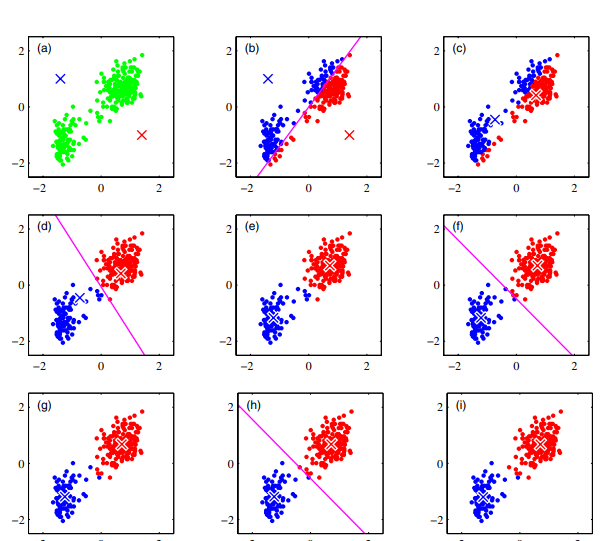
\includegraphics[width=0.40\textwidth]{2/figures/Kmeans.png}
    \caption{Ilustración de K-means. Fuente: \cite{bishop2006pattern}. \textit{Recuperado de Pattern Recognition and Machine Learning}.}
    \label{fig:kmeans}
\end{figure}


\subsection{Inercia en clustering}

En el análisis de clustering, la \textbf{inercia} es una medida de la dispersión interna de los datos dentro de un conjunto de clusters. En términos prácticos, la inercia cuantifica cuán estrechamente agrupados están los puntos de datos alrededor de los centroides de sus respectivos clusters. Esta medida es particularmente relevante en el algoritmo de \textit{K-means}, donde se busca minimizar la inercia para asegurar que cada cluster esté lo más compacto posible.

\subsubsection{Definición de inercia}

La inercia, también conocida como \textit{within-cluster sum of squares} (WCSS), se calcula como la suma de las distancias cuadradas entre cada punto de datos y el centroide de su cluster asignado. Matemáticamente, si tenemos un conjunto de datos \(X = \{x_1, x_2, \dots, x_n\}\) agrupado en \(k\) clusters \(C = \{C_1, C_2, \dots, C_k\}\), la inercia se define como:

\[
\text{Inercia} = \sum_{i=1}^{k} \sum_{x_j \in C_i} \| x_j - \mu_i \|^2
\]

donde:
\begin{itemize}
    \item \(C_i\) es el \(i\)-ésimo cluster,
    \item \(x_j\) representa cada punto de datos perteneciente al cluster \(C_i\),
    \item \(\mu_i\) es el centroide del cluster \(C_i\), calculado como el promedio de los puntos de datos dentro de \(C_i\),
    \item \(\| x_j - \mu_i \|\) es la distancia euclidiana entre el punto \(x_j\) y el centroide \(\mu_i\).
\end{itemize}

La inercia mide, por tanto, la compactación de los clusters: a menor inercia, mayor cohesión interna en cada cluster.

\subsubsection{Optimización de clusters mediante inercia}

La minimización de la inercia es uno de los objetivos principales en el algoritmo \textit{K-means}, ya que un valor bajo de inercia indica que los puntos de datos están más cerca de sus centroides, lo cual sugiere que los clusters son compactos y bien definidos. Sin embargo, la inercia tiende a disminuir a medida que se incrementa el número de clusters, lo que puede llevar a una sobreajuste si no se controla.

\subsubsection{Método del codo}

El \textbf{método del codo} es una técnica gráfica que utiliza la inercia para determinar el número óptimo de clusters en un conjunto de datos. Este método consiste en calcular la inercia para diferentes valores de \(k\) (número de clusters) y representar la inercia en función de \(k\). A medida que se aumenta \(k\), la inercia disminuye, ya que los clusters se vuelven más pequeños y específicos. Sin embargo, a partir de cierto punto, el beneficio de añadir clusters adicionales se reduce y la curva de inercia comienza a estabilizarse, formando un “codo”.

El punto donde se forma este “codo” en la gráfica indica el número de clusters óptimo. Elegir el valor de \(k\) en el codo permite obtener una buena estructura de clusters sin introducir clusters adicionales que solo disminuyan marginalmente la inercia.

\subsubsection{Ventajas de la Inercia}

La inercia ofrece una serie de beneficios al evaluar la calidad de los clusters:
\begin{itemize}
    \item \textbf{Cohesión de los clusters}: Minimizar la inercia asegura que los puntos dentro de cada cluster estén lo más cerca posible de sus centroides, lo que implica una alta cohesión interna.
    \item \textbf{Facilidad de interpretación}: La inercia es una medida intuitiva y directa para evaluar la dispersión de los datos, proporcionando una métrica clara para comparar diferentes agrupamientos.
    \item \textbf{Aplicabilidad en el Método del Codo}: La inercia es fundamental en el método del codo, que permite identificar de manera gráfica el número de clusters óptimo, optimizando así la estructura del agrupamiento.
\end{itemize}



\section{Marco Conceptual}
\subsection{Scraping}
Scraping es el proceso de extracción automática de información desde páginas web. Este método permite recopilar grandes volúmenes de datos de manera eficiente y organizada, especialmente útil en contextos donde se necesita obtener y estructurar datos no disponibles de forma directa en una API o base de datos. Para su implementación, se utilizan herramientas y librerías, como \texttt{BeautifulSoup} y \texttt{Selenium}, que facilitan la navegación y extracción de elementos específicos dentro de una página web, como textos, imágenes o enlaces. El scraping es particularmente relevante en el análisis de datos y la curaduría de contenido, ya que permite alimentar sistemas de análisis y machine learning con datos en tiempo real o en grandes cantidades.

\subsection{Automatización}
La automatización es el proceso de emplear tecnología para realizar tareas de forma autónoma, con mínima intervención humana. En el ámbito de procesamiento de datos y análisis de contenido, la automatización facilita la ejecución de procesos repetitivos y complejos, como la extracción y organización de grandes volúmenes de datos, mejorando tanto la precisión como la eficiencia. En el contexto de contenido audiovisual, la automatización permite aplicar algoritmos que identifican patrones y seleccionan datos relevantes sin necesidad de intervención manual en cada paso, asegurando que el sistema pueda manejar el flujo constante de información. Además, la automatización es fundamental para lograr consistencia en el tratamiento de los datos, reduciendo errores y tiempo en cada fase del proceso, desde la recolección de datos hasta la generación de resultados finales, optimizando el análisis en contextos de alta carga informativa.

\subsection{Curaduría de contenido}
La curaduría de contenido es un proceso que involucra la selección, organización y presentación de la información más relevante dentro de un amplio conjunto de datos. En el contexto de la información digital, la curaduría se convierte en una herramienta clave para filtrar y destacar elementos específicos que son de interés para el usuario. Esto es especialmente útil en medios audiovisuales, donde se busca identificar los momentos clave en grandes volúmenes de contenido para crear resúmenes informativos. La curaduría automatizada utiliza algoritmos y técnicas de machine learning para analizar y seleccionar segmentos de interés, optimizando así el consumo de información. Esta automatización de la curaduría también ayuda a personalizar la información en función de patrones específicos de uso, haciendo que la presentación del contenido sea más precisa y atractiva para audiencias específicas.

\subsection{Preprocesamiento de datos}
El preprocesamiento es una fase crítica en el análisis de datos, especialmente en el tratamiento de imágenes y videos. Involucra una serie de técnicas que mejoran la calidad de los datos y preparan el contenido visual para su posterior análisis. Entre los procesos de preprocesamiento comunes se incluyen la normalización de colores, que ajusta los valores de color para que sean coherentes en todas las imágenes; el redimensionado, que ajusta el tamaño de los frames; y la eliminación de ruido, que remueve elementos no deseados en los datos visuales. Estas técnicas permiten que los datos sean interpretados de manera uniforme por los algoritmos de aprendizaje automático, asegurando una mayor precisión y consistencia en el análisis de grandes volúmenes de información. El preprocesamiento también contribuye a reducir el tiempo de procesamiento, optimizando el flujo de trabajo en proyectos de análisis masivo.

\subsection{Extracción de características}
La extracción de características es el proceso mediante el cual se identifican y capturan los atributos visuales más representativos de una imagen o un video. Este proceso convierte el contenido visual en vectores de datos numéricos que pueden ser fácilmente manipulados y analizados por algoritmos de machine learning.

\subsection{Clustering}
El clustering es una técnica de aprendizaje no supervisado que organiza datos en grupos o clusters basados en sus similitudes. Esta técnica es particularmente útil en el análisis de contenido visual, donde el clustering permite agrupar frames de video que presentan características visuales similares, facilitando la identificación de segmentos relevantes en el contenido. El clustering ayuda a reducir la complejidad en el análisis de datos masivos, permitiendo una estructuración que optimiza la selección de frames clave y mejora la eficiencia de los resúmenes automáticos.

\subsection{Reducción de dimensionalidad}
La reducción de dimensionalidad es una técnica que simplifica la estructura de los datos, eliminando variables redundantes o irrelevantes sin perder la esencia de la información. En el contexto de análisis visual, la reducción de dimensionalidad permite optimizar el uso de los datos al extraer solo aquellas características que aportan mayor valor informativo. Esto no solo reduce el tiempo y recursos necesarios para el procesamiento, sino que también permite mejorar la precisión de los modelos de machine learning al reducir el ruido en los datos.

\subsection{Evaluación de clusters}
La evaluación de clusters es el proceso de analizar la calidad y coherencia de los grupos formados en un conjunto de datos, asegurando que los datos agrupados sean internamente homogéneos y estén bien diferenciados de otros clusters. En proyectos de análisis visual, la evaluación de clusters es crucial para garantizar que los grupos formados representen de manera precisa distintos segmentos del contenido. Esto permite optimizar la selección de frames clave y asegurar que el contenido sea adecuado para la creación de resúmenes automáticos.

\subsection{Selección de frames clave}
La selección de frames es el proceso de identificar y elegir momentos específicos o representativos de un video para su análisis posterior. Esta técnica permite reducir significativamente el número de frames que se deben procesar, optimizando el uso de recursos computacionales y mejorando la eficiencia en el análisis de contenido. La selección de frames clave se realiza en función de métricas de representatividad, permitiendo que los segmentos seleccionados reflejen de manera precisa los momentos importantes del video. En la creación de resúmenes automáticos, la selección de frames clave facilita la generación de una representación visual concisa sin perder detalles importantes.

\subsection{Metadatos}
Los metadatos son datos descriptivos que acompañan al contenido multimedia y proporcionan información adicional sobre el archivo, como su fecha de creación, duración, etiquetas y descripción. En el análisis de videos, los metadatos permiten organizar, buscar y filtrar contenido de manera estructurada, mejorando la accesibilidad y facilitando la clasificación y curaduría de contenido audiovisual. Los metadatos son fundamentales para gestionar grandes volúmenes de datos, ya que permiten una organización eficiente de la información y ofrecen contexto sobre cada archivo de video, facilitando su identificación y análisis.

\subsection{Etiquetado de datos}
El etiquetado de datos es el proceso de asignar identificadores o etiquetas a elementos de un conjunto de datos para facilitar su clasificación y análisis. En el caso de los frames de video, el etiquetado permite identificar y organizar los diferentes momentos en función de su contenido, ayudando a estructurar los datos para un análisis más eficiente.

\subsection{Concatenación de características}
El stacking de características es un proceso que combina múltiples vectores de características en una estructura unificada, permitiendo representar diversas propiedades de los datos de manera conjunta. En el análisis de contenido visual, el stacking permite integrar características obtenidas a través de diferentes métodos de extracción en una sola estructura. Esto mejora la riqueza descriptiva de los datos y optimiza la precisión de los algoritmos en tareas de clasificación y clustering, proporcionando al modelo una visión más completa de los patrones y atributos presentes en el contenido visual.


\subsection{Extracción de Frames}
La extracción de frames consiste en seleccionar imágenes de un video a intervalos específicos, lo que permite obtener una muestra representativa del contenido visual. Este proceso es crucial para análisis posteriores, ya que reduce el volumen de datos y facilita la manipulación de imágenes.

\subsection{Aplicación de Línea de Comando}
La aplicación de línea de comando permite ejecutar scripts y comandos específicos directamente en el sistema operativo. Esta técnica es útil en el procesamiento de datos y facilita la automatización de tareas como la descarga y organización de archivos en proyectos de gran escala.

\subsection{DataFrame}
El \textit{DataFrame} es una estructura de datos en formato tabular, que permite organizar y manejar grandes volúmenes de datos de manera eficiente. Cada columna puede contener diferentes tipos de datos, y esta organización es ideal para el análisis estructurado en proyectos de procesamiento de datos y machine learning.

\subsection{Concatenación de Videos}
La concatenación de videos es el proceso de unir varios segmentos de video en uno solo. Este procedimiento es particularmente útil para crear resúmenes visuales de clips relevantes, permitiendo una presentación continua de los eventos clave sin interrupciones.



\chapter{METODOLOGÍA DE LA INVESTIGACIÓN}
\section{Diseño de la investigación}

En este segmento del documento se explica cual fue el tipo y enfoque del trabajo de
investigación, al igual que la población y la muestra. 

\subsection{Tipo de Investigación}
El diseño del presente trabajo de investigación es de tipo no experimental, ya que no se manipulan las variables independientes y se observa su relación en el contexto de la implementación de un modelo de traducción de lenguaje de señas utilizando técnicas de Deep Learning. La etapa inicial del trabajo involucra el análisis de vídeos de lenguaje de señas, los cuales serán procesados mediante técnicas de Deep Learning. \\

El nivel del presente trabajo de investigación es explicativo, dado que se enfoca en la implementación de un modelo de traducción de lenguaje de señas utilizando Deep Learning para personas con discapacidad del habla. El objetivo es determinar cómo se puede lograr la traducción efectiva del lenguaje de señas a texto y viceversa, estableciendo una relación entre los gestos y movimientos específicos del lenguaje de señas y su correspondencia con el texto escrito. \\



\subsection{Enfoque de Investigación}

El enfoque del presente trabajo de investigación es cuantitativo, dado que se basa en la utilización de instrumentos para la identificación y medición del lenguaje de señas a través de técnicas de visión computacional. Estas técnicas proporcionarán resultados numéricos que, tras un análisis estadístico, servirán como entrada para implementar modelos de Deep Learning. 



\section{Población y muestra}

\begin{table}[h!]
	\centering
	\caption{Descripción del Estudio}
	\begin{tabular}{|>{\raggedright\arraybackslash}m{3cm}|>{\raggedright\arraybackslash}m{10cm}|}
		\hline
		\textbf{Categoría} & \textbf{Descripción} \\ \hline
		\textbf{Población} & Personas con discapacidades del habla y del escucha. \\ \hline
		\textbf{Muestra} & 
		\begin{itemize}
			\item 260 vídeos MP4 de diálogos en lenguaje de señas extraídas de Universidad Pontificia Universidad Católica del Perú.
			\item 355 vídeos MP4 de narración de historias en lenguaje de señas extraídas de Universidad Pontificia Universidad Católica del Perú.
			\item 103 vídeos MP4 de nombres, estados y acciones en lenguaje de señas extraídas de Universidad Pontificia Universidad Católica del Perú.
		\end{itemize}
		\\ \hline
		\textbf{Unidad de análisis} & Un vídeo de una persona comunicándose con lenguaje de señas \\ \hline
	\end{tabular}
\end{table}


\section{Operacionalización de Variables}

\begin{table}[h!]
	\centering
	\caption{Operacionalización de Variables}
	\begin{tabular}{|>{\raggedright\arraybackslash}m{4cm}|>{\raggedright\arraybackslash}m{4cm}|>{\raggedright\arraybackslash}m{4cm}|>{\raggedright\arraybackslash}m{4cm}|}
		\hline
		\textbf{Variable} & \textbf{Dimensión} & \textbf{Indicador} & \textbf{Cálculo} \\ \hline
		\textbf{Independiente: Modelo Deep Learning} 
		& Base de datos & Volumen de datos & Cantidad de videos MP4\\ \cline{2-4}
		
		\textbf{Dependiente: Traducción de Lenguaje de señas peruano para personas con discapacidades del habla} 
		& Indicadores de rendimiento de modelo & Precisión, recall, F1-score & Fórmulas \\ \hline
	\end{tabular}
\end{table}

\section{Técnicas de recolección}
	
	La base de datos se compone de vídeos en formato MP4 proporcionados por la Universidad Pontificia Universidad Católica del Perú. Estos vídeos fueron seleccionados por su relevancia y calidad para el estudio del lenguaje de señas. Los videos MP4 contienen diálogos, narraciones de historias, y nombres, estados y acciones en lenguaje de señas.


\section{Técnicas para el procesamiento y análisis de la información}

\subsection{Metodología de la implementación de la solución}

\subsubsection{Recolección de Datos}
La recolección de datos es una fase crítica en cualquier proyecto de Deep Learning. En esta tesis, se han recopilado un total de 718 vídeos MP4 de lenguaje de señas, extraídos de la Pontificia Universidad Católica del Perú. Los datos se dividen en tres categorías principales:
\begin{itemize}
	\item \textbf{260 vídeos MP4 de diálogos en lenguaje de señas}: Estos vídeos contienen conversaciones entre dos o más personas utilizando lenguaje de señas.
	\item \textbf{355 vídeos MP4 de narración de historias en lenguaje de señas}: En estos vídeos, las personas narran historias completas usando lenguaje de señas.
	\item \textbf{103 vídeos MP4 de nombres, estados y acciones en lenguaje de señas}: Estos vídeos muestran la señalización de nombres, estados emocionales y diversas acciones.
\end{itemize}

\subsubsection{Preprocesamiento de Datos}
El preprocesamiento de datos es una etapa esencial para preparar los datos brutos para ser utilizados por los modelos de Deep Learning. Las tareas de preprocesamiento incluyen:
\begin{itemize}
	\item \textbf{Extracción de Frames}: Se extraen frames de los vídeos a intervalos regulares para capturar las diferentes poses y movimientos de las manos.
	\item \textbf{Aumento de Datos}: Se aplican técnicas de aumento de datos, como rotación, escalado y traslación, para aumentar la variabilidad y robustez del conjunto de datos.
	\item \textbf{Etiquetado}: Cada frame o secuencia de frames se etiqueta con la correspondiente señal del lenguaje de señas que representa.
	\item \textbf{Normalización}: Los frames se normalizan para asegurarse de que todos los datos tengan el mismo formato y escala.
\end{itemize}

\subsubsection{Uso de Redes Neuronales Convolucionales (CNN)}
Las redes neuronales convolucionales (CNN) son efectivas para la tarea de reconocimiento de imágenes y, en este caso, para la identificación de señales en los frames extraídos de los vídeos. Las etapas clave incluyen:
\begin{itemize}
	\item \textbf{Diseño de la Arquitectura CNN}: Se diseña una arquitectura de CNN adecuada para la tarea, con capas convolucionales, de pooling y totalmente conectadas.
	\item \textbf{Entrenamiento}: La CNN se entrena utilizando los datos preprocesados, ajustando los pesos de la red para minimizar el error en la predicción de las señales.
	\item \textbf{Validación}: Se valida el rendimiento de la CNN utilizando un conjunto de datos de validación separado, ajustando los hiperparámetros según sea necesario.
\end{itemize}

\subsubsection{Integración de LSTM}
Las redes neuronales de memoria a largo plazo (LSTM) son ideales para manejar secuencias de datos y capturar dependencias temporales. En esta fase:
\begin{itemize}
	\item \textbf{Extracción de Secuencias}: Se crean secuencias de frames para capturar el movimiento y la continuidad de las señales.
	\item \textbf{Diseño de la Arquitectura LSTM}: Se diseña una arquitectura LSTM que pueda procesar las secuencias de frames y capturar las dependencias temporales entre ellos.
	\item \textbf{Entrenamiento del Modelo}: El modelo LSTM se entrena para aprender las transiciones y la continuidad de las señales en las secuencias de frames.
	\item \textbf{Combinación con CNN}: La salida de la CNN se combina con la LSTM para mejorar la precisión en la predicción de señales.
\end{itemize}

\subsubsection{Evaluación del Modelo}
La evaluación del modelo es crucial para determinar su eficacia y áreas de mejora. Las actividades incluyen:
\begin{itemize}
	\item \textbf{Métricas de Evaluación}: Se utilizarán métricas como Recall, F1-Score y Accuracy para evaluar el rendimiento del modelo.
	\item \textbf{Pruebas con Datos de Prueba}: Se prueba el modelo con un conjunto de datos de prueba que no se ha utilizado durante el entrenamiento para evaluar su rendimiento en datos no vistos.
	\item \textbf{Análisis de Errores}: Se realiza un análisis de errores para identificar patrones comunes en las predicciones incorrectas y mejorar el modelo.
	\item \textbf{Ajustes y Mejoras}: Basado en los resultados de la evaluación, se ajustan los hiperparámetros y se realizan mejoras en la arquitectura del modelo para aumentar su rendimiento.
\end{itemize}

\begin{figure}[h!]
	\centering
	\includegraphics[width=1\textwidth]{3/figures/Metodología.png}
	\caption{Metodología Iterativa}
	\label{fig:etiqueta_de_la_figura}
\end{figure}


\subsection{Metodología para la medición de resultados}

\subsection*{Accuracy}
El accuracy medirá la proporción de predicciones correctas sobre el total de predicciones realizadas por el modelo Deep Learning. Se utilizará para obtener una visión general del rendimiento del modelo.
\begin{equation}
	\text{Accuracy} = \frac{TP + TN}{TP + TN + FP + FN}
\end{equation}

\subsection*{Recall}
El Recall medirá la capacidad del modelo para identificar correctamente todas las instancias positivas.
\begin{equation}
	\text{Recall} = \frac{TP}{TP + FN}
\end{equation}

\subsection*{F1-Score}
Se utilizará en caso el modelo presente un desequilibrio entre las clases y se necesita un equilibrio tanto en el Accuracy como en el recall.
\begin{equation}
	\text{F1-Score} = 2 \cdot \frac{\text{Precision} \cdot \text{Recall}}{\text{Precision} + \text{Recall}}
\end{equation}


\section{Cronograma de actividades}
\begin{figure}[h!]
	\centering
	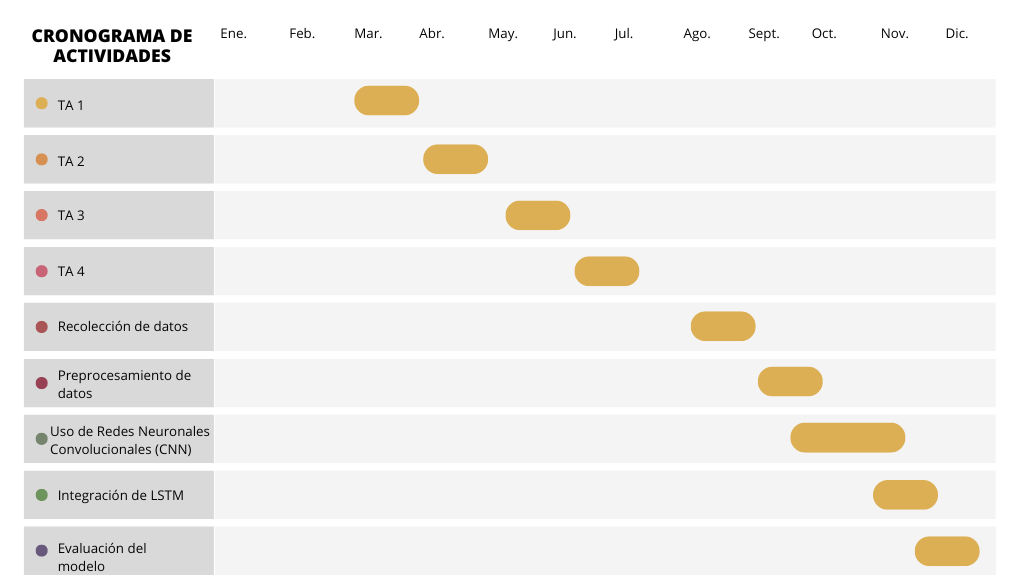
\includegraphics[width=1\textwidth]{3/figures/Actividades.png}
	\caption{Metodología Iterativa}
	\label{fig:etiqueta_de_la_figura}
\end{figure}
\section{Presupuesto}


\begin{table}[h!]
	\centering
	\caption{Presupuesto del Proyecto}
	\begin{tabular}{|>{\raggedright\arraybackslash}m{10cm}|>{\raggedright\arraybackslash}m{4cm}|}
		\hline
		\textbf{Item} & \textbf{Costo (Soles)} \\ \hline
		Laptop & 3500 \\ \hline
		Cámara & 250 \\ \hline
		\textbf{Total} & \textbf{3750} \\ \hline
	\end{tabular}
\end{table}
%\chapter{DESARROLLO DE LA SOLUCIÓN}

Este capítulo describe el desarrollo técnico y metodológico aplicado para llevar a cabo el análisis de los datos en este proyecto. Cada sección detalla los pasos realizados, las herramientas empleadas y los enfoques metodológicos utilizados para lograr una representación visual y analítica de los datos de video obtenidos.

\section{Equipo utilizado}
A continuación se presenta una descripción detallada de las características del equipo de cómputo utilizado en el desarrollo del proyecto. Esto es relevante para replicar el análisis en condiciones similares.

\begin{table}[H]
    \centering
    \caption{Especificaciones del equipo utilizado}
    \begin{tabular}{p{5cm} p{8cm}} \hline
        \textbf{Característica} & \textbf{Especificación} \\ \hline
        Nombre del dispositivo & LAPTOP-OSCAR \\
        Procesador & AMD Ryzen 7 6800H con Radeon Graphics, 3.20 GHz \\
        RAM instalada & 16.0 GB (15.3 GB utilizable) \\
        Tipo de sistema & Sistema operativo de 64 bits, procesador basado en x64 \\
        Sistema operativo & Windows \\ \hline
    \end{tabular}
    \label{tabla:laptop}
\end{table}
\section{Especificaciones de Python}
Para este proyecto se utilizó la versión 3.12.4 de Python, cuyo entorno fue configurado para cumplir con los requisitos de las bibliotecas y módulos necesarios.

\begin{table}[H]
    \centering
    \caption{Especificaciones de Python utilizado}
    \begin{tabular}{p{5cm} p{8cm}} \hline
        \textbf{Característica} & \textbf{Especificación} \\ \hline
        Versión de Python & 3.12.4 \\
        Fecha de compilación & 6 de junio de 2024 \\ \hline
    \end{tabular}
    \label{tabla:python}
\end{table}

\section{Librerías}
Las librerías descritas a continuación fueron esenciales para las distintas etapas de procesamiento, análisis y visualización en este proyecto.

\begin{longtable}{p{4cm} p{11cm}}
    \caption{Descripción de Librerías Usadas en el Proyecto} \\ % Caption con numeración automática
    \hline
    \textbf{Librería} & \textbf{Descripción} \\
    \hline
    \endfirsthead
    
    \hline
    \textbf{Librería} & \textbf{Descripción} \\
    \hline
    \endhead
    
    \hline
    \endfoot
    
    \hline
    \endlastfoot
    
    \multicolumn{2}{c}{\textbf{Web Scraping y automatización}} \\
    \hline
    \texttt{time} & Proporciona funciones para gestionar el tiempo, como retrasos y mediciones de intervalos, útiles en sincronización de procesos y espera entre solicitudes. \\
    \texttt{os} & Facilita la interacción con el sistema operativo, como gestionar archivos y directorios, útil en automatización. \\
    \texttt{subprocess} & Ejecuta comandos del sistema desde Python, permitiendo interactuar con otros programas o scripts. \\
    \texttt{psutil} & Ofrece una interfaz para monitorear recursos del sistema (CPU, memoria) y gestionar procesos en segundo plano. \\
    \texttt{selenium} & Herramienta para automatización de navegadores, ideal para pruebas web y scraping de sitios dinámicos. \\
    \texttt{tqdm} & Crea barras de progreso en loops, útil para monitorear procesos largos. \\
    \hline
    
    \multicolumn{2}{c}{\textbf{Procesamiento de datos}} \\
    \hline
    \texttt{numpy} & Biblioteca fundamental para operaciones matemáticas y estructuras de datos de alto rendimiento, como arreglos multidimensionales. \\
    \texttt{pandas} & Ofrece estructuras de datos como DataFrames, ideales para manipulación y análisis de datos tabulares. \\
    \hline
    
    \multicolumn{2}{c}{\textbf{Procesamiento de imágenes}} \\
    \hline
    \texttt{cv2} & OpenCV, biblioteca de visión artificial para procesamiento y análisis de imágenes y video, común en proyectos de visión. \\
    \texttt{hog} & Función en \texttt{skimage.feature} para extracción de características en imágenes usando Histogramas de Gradientes Orientados (HOG). \\
    \hline
    
    \multicolumn{2}{c}{\textbf{Redes neuronales y Deep learning}} \\
    \hline
    \texttt{ResNet50} & Arquitectura de red preentrenada, común para extracción de características y clasificación en imágenes. Se importa desde \texttt{tensorflow.keras.applications}. \\
    \texttt{preprocessing} & Módulo en Keras para preprocesamiento de datos e imágenes, útil en preparación de datos para redes neuronales. \\
    \texttt{models} & API de Keras para crear y gestionar modelos, permitiendo el diseño de redes neuronales profundas. \\
    \hline
    
    \multicolumn{2}{c}{\textbf{Clustering y Machine learning}} \\
    \hline
    \texttt{KMeans} & Algoritmo de agrupamiento en \texttt{sklearn.cluster}, útil para clasificar datos en grupos similares. \\
    \texttt{metrics} & Módulo de \texttt{sklearn} que ofrece métricas para evaluar modelos y métodos de clustering. \\
    \texttt{PCA} & Método de reducción de dimensionalidad en \texttt{sklearn.decomposition}, que simplifica conjuntos de datos complejos. \\
    \hline
    
    \multicolumn{2}{c}{\textbf{Visualización}} \\
    \hline
    \texttt{matplotlib} & Biblioteca principal para visualización de datos, permite crear gráficos de varios tipos en Python. \\
    \hline
    
\end{longtable}



\section{Extracción de datos}

La extracción de datos fue un paso fundamental en este proyecto, ya que permitió obtener información relevante de videos publicados en YouTube para su posterior análisis. El proceso se llevó a cabo en diferentes etapas que abarcaron desde la recopilación de los enlaces de los videos, la descarga de los mismos, hasta la extracción de frames que fueron utilizados para generar descriptores de características mediante técnicas de visión computacional.

\subsection{Automatización de la búsqueda de videos en YouTube}

Para obtener los videos de interés, se realizó una búsqueda automatizada en YouTube utilizando la librería \texttt{Selenium}. El objetivo era filtrar noticias en vivo y limitar la cantidad de videos a descargar. La siguiente secuencia de pasos describe el proceso:

\begin{itemize}
    \item Se inició una sesión de navegador automatizada con Selenium, controlando el navegador Chrome.
    \item A través de interacciones programadas, se realizaron búsquedas con palabras clave específicas y se aplicaron filtros para obtener resultados de videos de un único día y de la duración suficiente.
    \item Los enlaces de los videos obtenidos fueron almacenados en una lista para ser descargados posteriormente.
\end{itemize}

\begin{figure}[H]
    \centering
    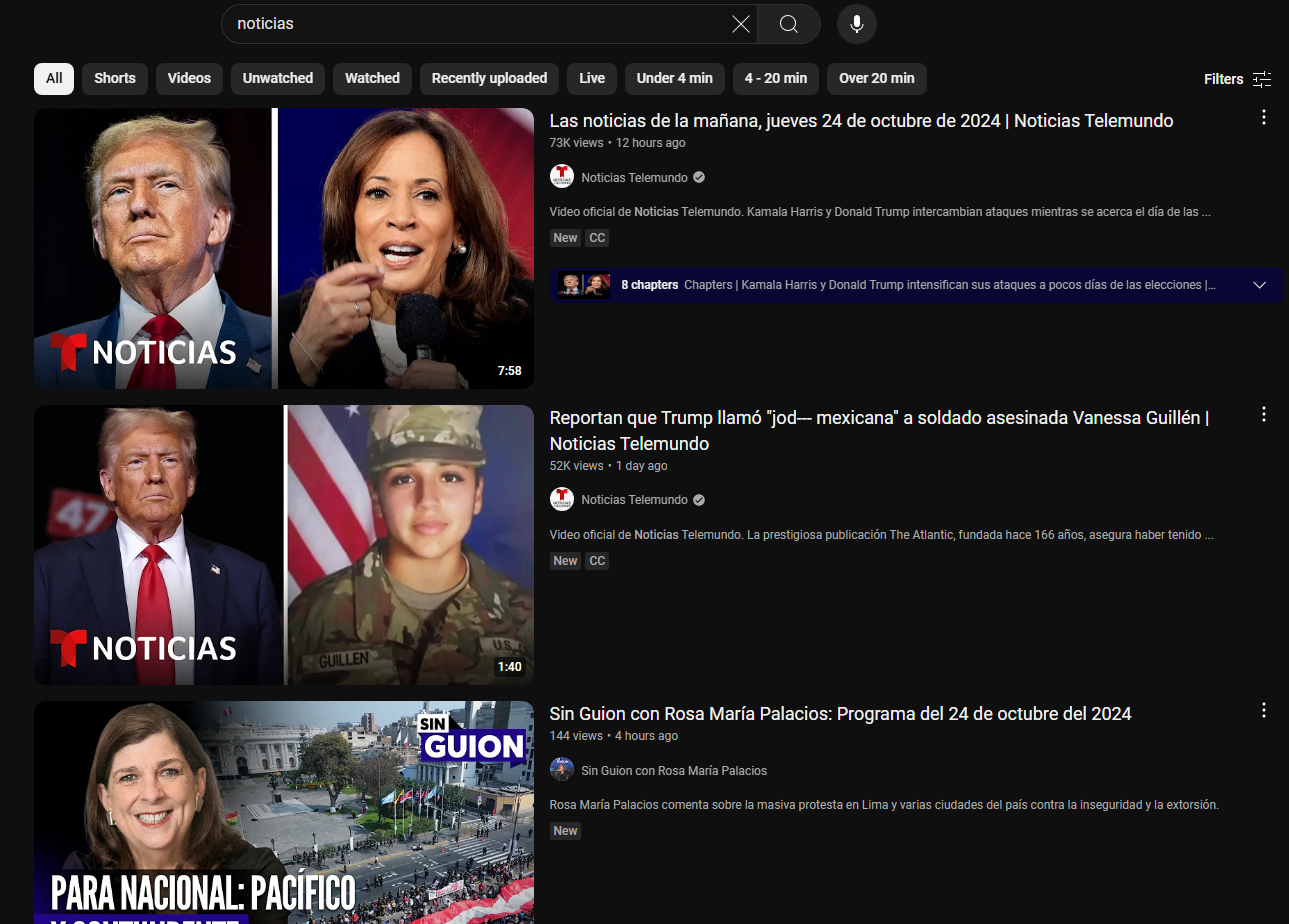
\includegraphics[width=0.70\textwidth]{4/figures/Extraccion_1.png}
    \caption{Página de partida de scrapping.}
    \label{fig:convolucion}
\end{figure}

\begin{figure}[H]
    \centering
    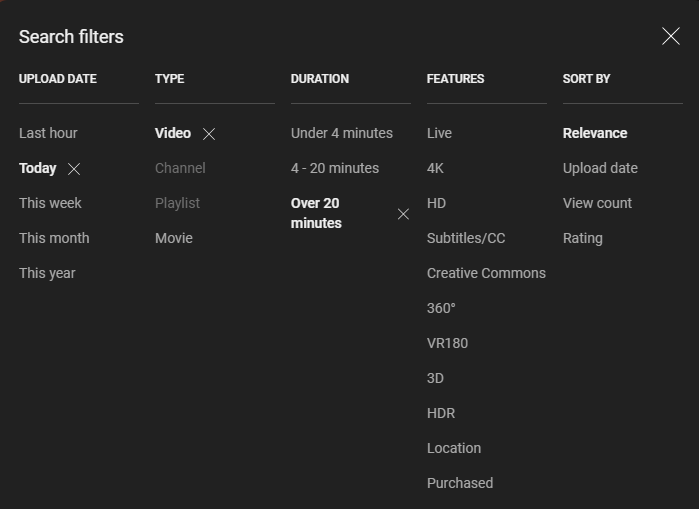
\includegraphics[width=0.70\textwidth]{4/figures/Extraccion_3.png}
    \caption{Filtros aplicados a los resultados de video.}
    \label{fig:convolucion}
\end{figure}

\subsection{Descarga de videos}

Para la recopilación de datos, se automatizó la descarga de videos de YouTube que cumplieran con los criterios. Para ello, se utilizó la herramienta \texttt{yt-dlp} estableciéndole los parámetros de descarga necesarios como el tamaño máximo de archivo y la calidad del video establecida en 720p.

El código de descarga inicializa una lista de enlaces de YouTube y ejecuta la descarga de cada video de forma secuencial, con un intervalo entre descargas para evitar bloqueos por parte de YouTube. A continuación, se detallan las opciones clave usadas con \texttt{yt-dlp}:

\begin{itemize}
    \item \texttt{--format "bestvideo[height<=720]"}: Especifica que se descargue la mejor calidad de video disponible con una altura máxima de 720 píxeles.
    \item \texttt{--max-filesize 400M}: Establece un tamaño máximo de archivo de 400 MB para evitar descargas excesivamente grandes.
\end{itemize}


\begin{figure}[H]
    \centering
    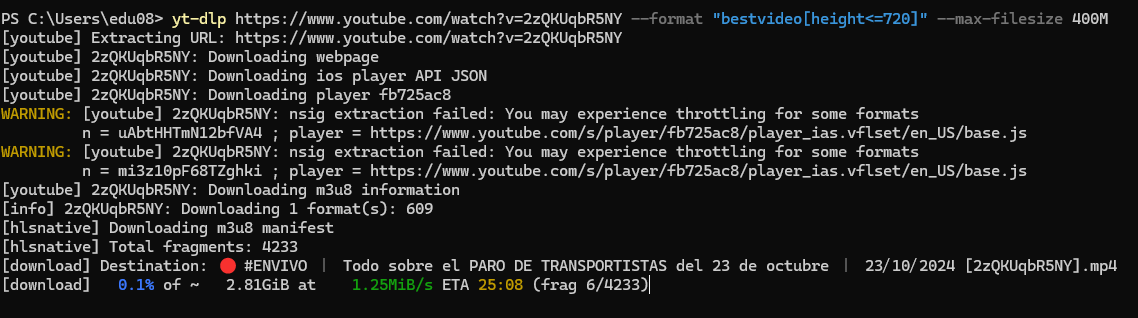
\includegraphics[width=0.90\textwidth]{4/figures/Descarga_1.png}
    \caption{Instrucción de descarga de video.}
    \label{fig:convolucion}
\end{figure}

\subsection{Organización de videos}

Para organizar los videos descargados, se empleó un script que clasifica los archivos en función de su tipo y ubicación en directorios específicos. Este proceso permite gestionar eficientemente los archivos de video y eliminar los archivos no necesarios generados durante la descarga. El procedimiento se detalla a continuación.

\begin{enumerate}
    \item \textbf{Creación del directorio de videos:} Inicialmente, se define un directorio específico para almacenar los archivos de video. Si la carpeta de destino no existe, el código se encarga de crearla utilizando el comando \texttt{os.makedirs}.
    
    \item \textbf{Clasificación de archivos:} Se definen las extensiones de archivo de video permitidas (\texttt{.mp4} y \texttt{.part}), las cuales son revisadas en cada archivo del directorio actual. Cualquier archivo con una de estas extensiones se mueve al directorio de videos.
    
    \item \textbf{Eliminación de archivos no necesarios:} Cualquier archivo que no corresponda a un video o al archivo \texttt{Tesis.ipynb} (notebook principal) es eliminado del directorio, optimizando el espacio y reduciendo el desorden en el sistema de archivos.
\end{enumerate}

Este proceso automatizado mejora la organización del proyecto y asegura que solo los archivos relevantes se mantengan en el directorio principal. En la investigación se obtuvieron 1.79 GB de contenido dividido en 15 videos de noticias.

\begin{figure}[H]
    \centering
    \includegraphics[width=0.40\textwidth]{4/figures/Organzación_1.png}
    \caption{Descripción final de carpeta de videos a procesar.}
    \label{fig:convolucion}
\end{figure}

\section{Preprocesamiento de datos}

El preprocesamiento de datos es un paso fundamental en este proyecto y consiste en cuatro etapas principales: la extracción de frames, el etiquetado de frames y las operaciones de transformación de los frames. Estas etapas permiten obtener representaciones visuales homogéneas y estructuradas, facilitando el análisis posterior mediante técnicas de machine learning.

\subsection{Extracción de frames}

La primera etapa del preprocesamiento es la extracción de frames de los videos. Los videos almacenados en la carpeta de entrada se procesan para obtener un conjunto de imágenes a intervalos de tiempo específicos, lo que permite captar información visual a lo largo de la duración del video. La extracción de frames se realiza a una tasa de \texttt{1 frame por segundo}, lo cual proporciona una representación balanceada entre resolución temporal y carga de procesamiento. Este proceso se logra utilizando la biblioteca \texttt{OpenCV}.

\subsection{Etiquetado de frames}

Cada frame extraído se etiqueta de manera única para mantener una referencia clara de su video de origen y posición temporal. La nomenclatura de los frames es de la forma \texttt{Video\{número\}\_Frame\{número\}.png}, donde:
\begin{itemize}
    \item \texttt{Video\{número\}} hace referencia al identificador del video de origen.
    \item \texttt{Frame\{número\}} indica el número de frame dentro del video.
\end{itemize}

Esta estructura de nombres facilita el seguimiento de cada frame y permite una asociación directa entre la imagen y el video de origen. En etapas posteriores se hará uso de la etiqueta para la identificación de frames clave y la generación de clips.

\begin{figure}[H]
    \centering
    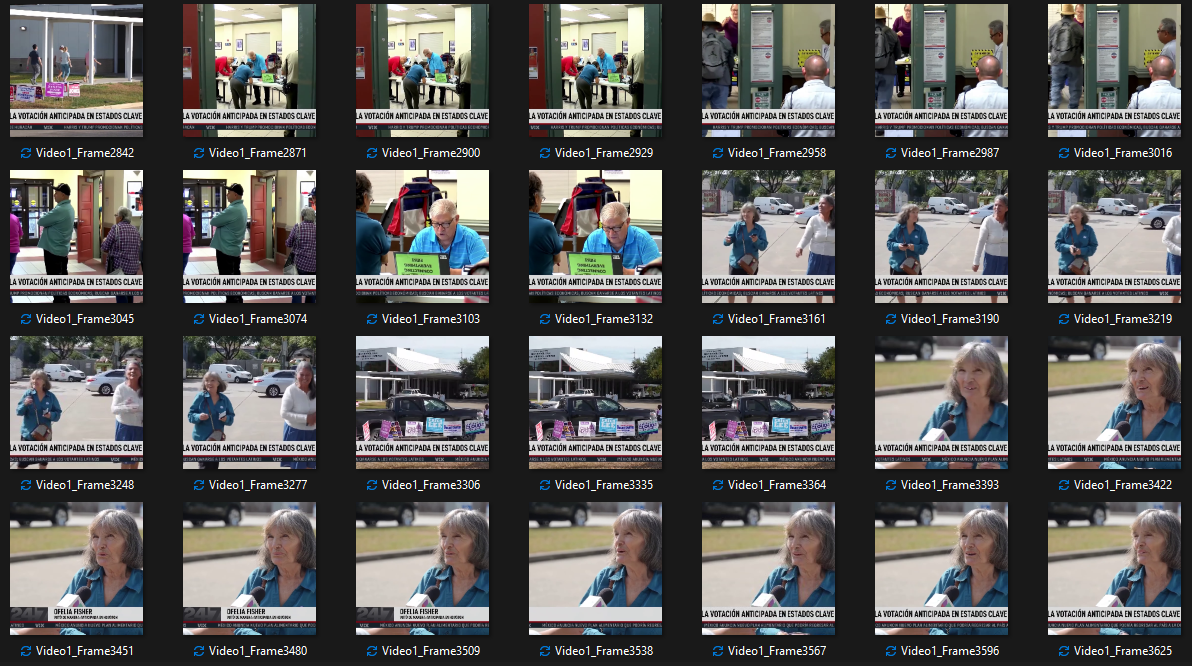
\includegraphics[width=0.80\textwidth]{4/figures/Etiquetado_1.png}
    \caption{Frames etiquetados en la carpeta de frames.}
    \label{fig:convolucion}
\end{figure}

\subsection{Operaciones sobre los frames}

Para garantizar la uniformidad en los datos y preparar los frames para su posterior análisis, cada imagen extraída de los videos pasa por un proceso de redimensión y recorte. Estos ajustes son esenciales para normalizar el tamaño de los frames y preservar la proporción original de la imagen, evitando así posibles distorsiones que puedan afectar los resultados en etapas posteriores del procesamiento.

El tamaño final de cada frame se define en \texttt{224x224 píxeles}, un formato ampliamente compatible con redes neuronales convolucionales (CNNs) y modelos de aprendizaje profundo en general. Este proceso de preprocesamiento se realiza en dos pasos clave:

\begin{itemize}
    \item \textbf{Redimensión}: Inicialmente, la imagen es escalada para que su dimensión menor (ancho o alto) se ajuste al tamaño objetivo de \texttt{224 píxeles}. Esto asegura que la imagen completa se mantenga dentro del marco sin deformaciones y preservando la proporción de los elementos visuales originales.
    \item \textbf{Recorte}: Una vez redimensionada, la imagen es recortada para ajustar la dimensión restante a \texttt{224 píxeles}, logrando así un encuadre preciso sin distorsionar los contenidos importantes. 
\end{itemize}


\begin{figure}[H]
    \centering
    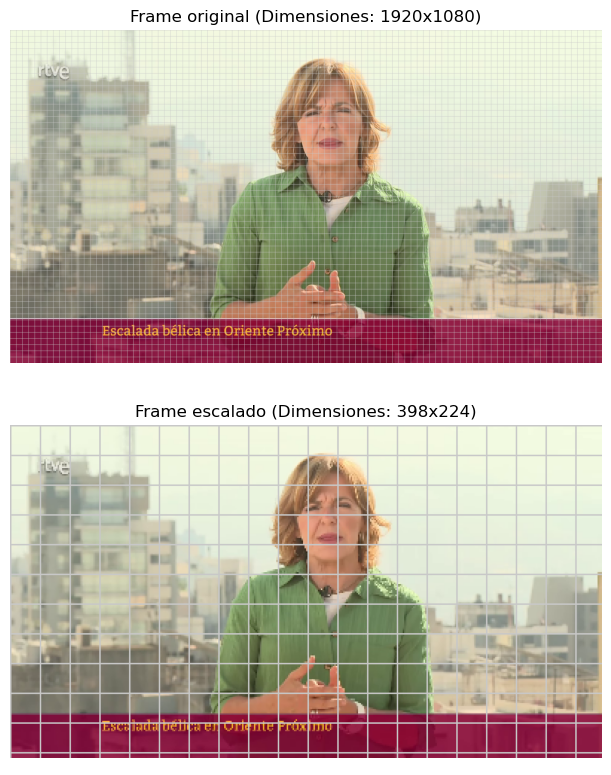
\includegraphics[width=0.50\textwidth]{4/figures/Preprocesamiento_1.png}
    \caption{Proceso de redimensión de la imagen.}
    \label{fig:preproc-resize}
\end{figure}

La Figura~\ref{fig:preproc-resize} ilustra la etapa de redimensión, mientras que la Figura~\ref{fig:preproc-crop} muestra el proceso de recorte, donde se enmarca la sección central de la imagen para asegurar consistencia en el análisis de los frames.

\begin{figure}[H]
    \centering
    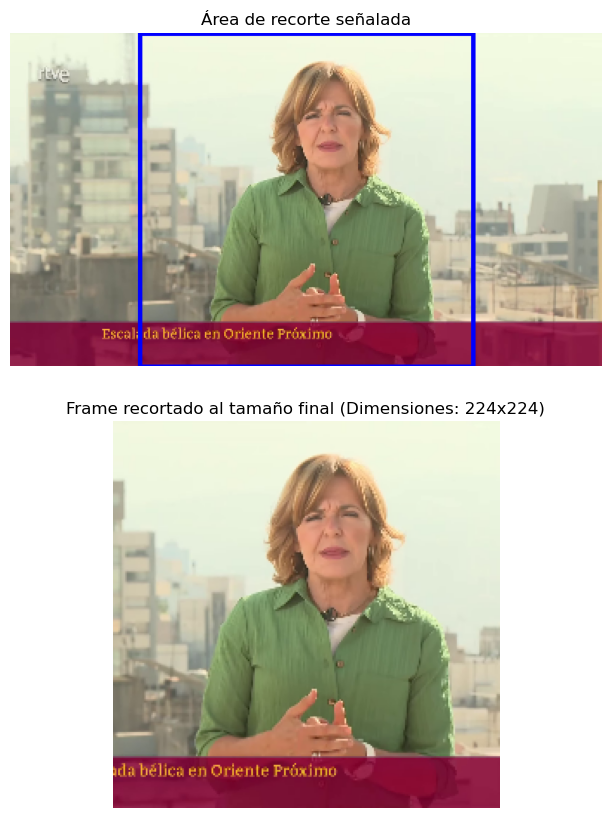
\includegraphics[width=0.30\textwidth]{4/figures/Preprocesamiento_2.png}
    \caption{Proceso de recorte de la imagen.}
    \label{fig:preproc-crop}
\end{figure}



\subsection{Guardado de frames}

Finalmente, los frames procesados se almacenan en un directorio de salida específico, asegurando que cada imagen esté etiquetada de forma clara y sea fácilmente localizable para su análisis posterior. Los frames resultantes se guardan en formato \texttt{.png}, manteniendo una alta calidad de imagen sin compresión excesiva que podría comprometer la precisión en las etapas de análisis.

\begin{figure}[H]
    \centering
    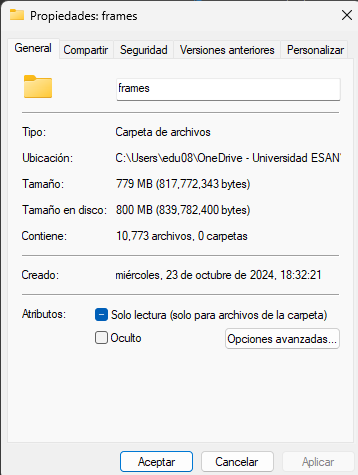
\includegraphics[width=0.40\textwidth]{4/figures/Guardado_1.png}
    \caption{Características principales de la carpeta de frames generada.}
    \label{fig:convolucion}
\end{figure}

Este proceso generó más de 10000 frames uniformes y etiquetados listos para el proceso de Extracción de características.

\section{Extracción de características}
La extracción de características es esencial para la representación compacta de la información visual en imágenes, permitiendo la realización de tareas analíticas avanzadas. En esta sección se describen los métodos de extracción y combinación de características utilizados: Histogram of Oriented Gradients (HOG) y Convolutional Neural Networks (CNN) con el modelo ResNet50 preentrenado en ImageNet, y el proceso de concatenación para unir las características de ambas técnicas.

\subsection{HOG (Histogram of Oriented Gradients)}

El método HOG se implementa en este proyecto como una técnica avanzada de extracción de características visuales, transformando cada frame en histogramas de gradientes de orientación. Este enfoque permite identificar contornos y texturas esenciales en los datos de imagen, evitando la necesidad de redundar en descripciones del proceso detallado, el cual ya ha sido expuesto en la sección teórica sobre \textit{extracción de características} (ver sección \ref{sec:preprocesamiento_imagenes}). En esta fase de análisis, HOG contribuye de manera significativa al modelado de patrones visuales, resultando especialmente efectivo en la representación de información estructural crítica para el análisis de patrones y el agrupamiento de datos visuales.

La Figura~\ref{fig:preproc-crop} ilustra el proceso de conversión de cada imagen en un descriptor HOG, enfatizando la metodología aplicada para generar estos histogramas de gradientes orientados que sintetizan las características visuales fundamentales de cada frame. 

\begin{figure}[H]
    \centering
    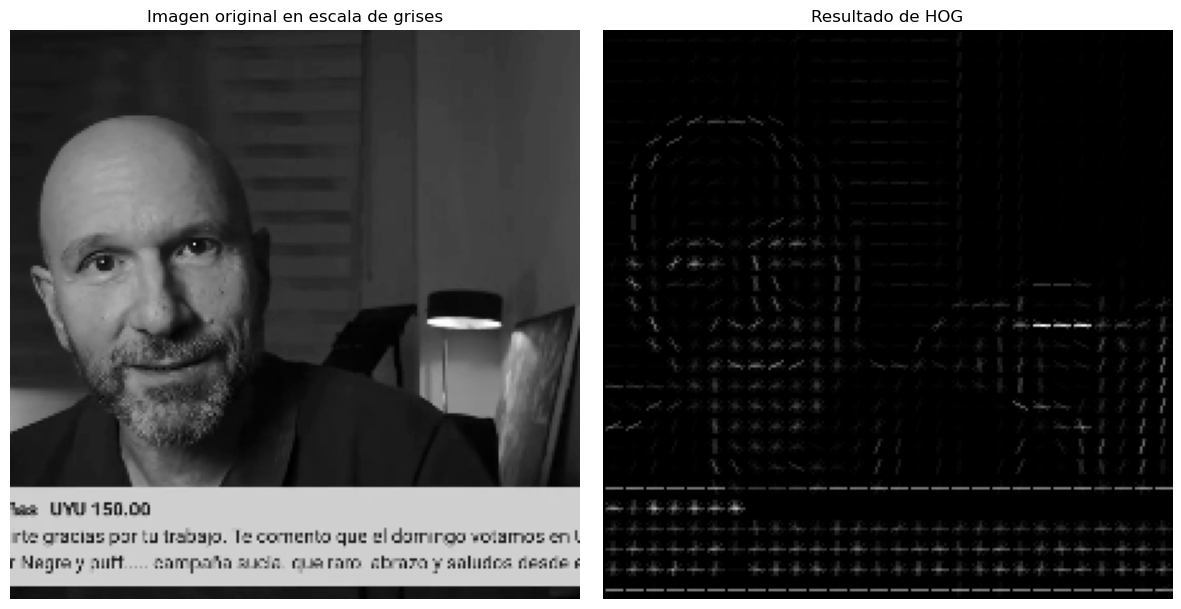
\includegraphics[width=0.60\textwidth]{4/figures/HOG_1.png}
    \caption{Proceso de transformación de imagen utilizando HOG.}
    \label{fig:preproc-crop}
\end{figure}

Los descriptores HOG obtenidos se integran en un \texttt{DataFrame}, el cual vincula cada frame con su correspondiente vector de características. Esta estructura, mostrada en la Figura~\ref{fig:convolucion}, no solo facilita la organización y accesibilidad de los datos, sino que también optimiza el procesamiento subsecuente. Al estructurar los datos en un formato tabular, el \texttt{DataFrame} permite un análisis más eficiente y la implementación de técnicas de machine learning en etapas posteriores del proyecto, asegurando una base de datos visualmente rica y ordenada para las siguientes fases del análisis.

\begin{figure}[H]
    \centering
    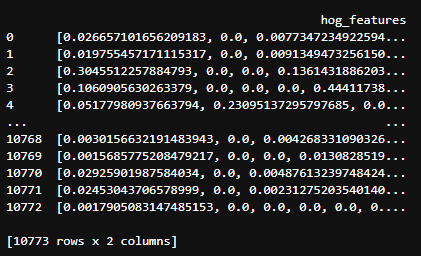
\includegraphics[width=0.60\textwidth]{4/figures/Caracteristicas_1.png}
    \caption{Estructura del DataFrame con los vectores de características HOG generados.}
    \label{fig:convolucion}
\end{figure}


\subsection{Extracción de características con CNN}
Para complementar la extracción HOG, se utiliza un modelo convolucional preentrenado (ResNet50) para extraer características de nivel más alto que capturan información estructural y semántica. la función extrae el vector de características de la capa \texttt{avg\_pool}, produciendo un descriptor de características CNN.

\begin{figure}[H]
    \centering
    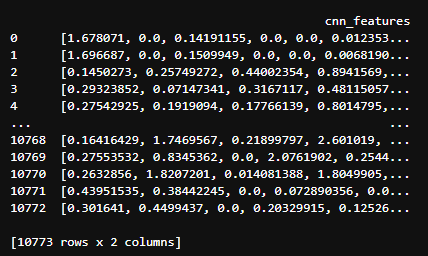
\includegraphics[width=0.60\textwidth]{4/figures/Caracteristicas_2.png}
    \caption{Dataframe generado por la red convolucional entrenada.}
    \label{fig:convolucion}
\end{figure}

\subsection{Concatenación de características}
Para maximizar la información obtenida a través de HOG y CNN, los vectores de características de ambas técnicas se integran en un único vector mediante un proceso de concatenación. Esta integración se realiza alineando ambos conjuntos de características de acuerdo con el identificador del frame y concatenando los vectores en una nueva columna denominada \texttt{combined\_features} dentro del \texttt{DataFrame} final, generando así una representación robusta de cada frame.

\begin{figure}[H]
    \centering
    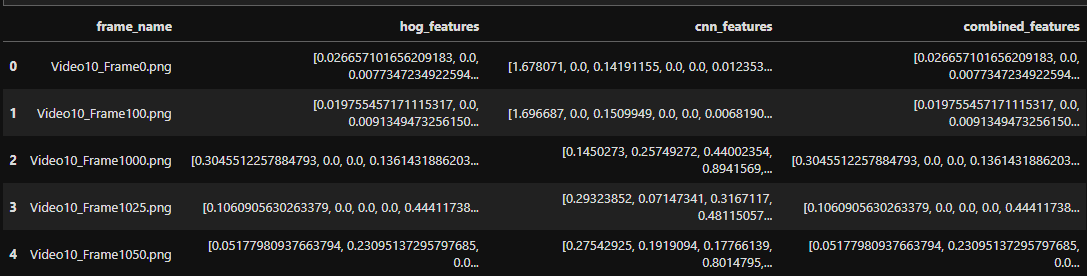
\includegraphics[width=0.70\textwidth]{4/figures/Caracteristicas_3.png}
    \caption{Concatenación de los vectores de características.}
    \label{fig:convolucion}
\end{figure}

Este \texttt{DataFrame} resultante, \texttt{merged\_df}, incluye las siguientes columnas:
\begin{itemize}
    \item \textbf{frame\_name}: El nombre del frame correspondiente.
    \item \textbf{hog\_features}: El vector de características HOG extraído.
    \item \textbf{cnn\_features}: El vector de características CNN extraído.
    \item \textbf{combined\_features}: Un vector de características unificado que contiene tanto HOG como CNN, lo que proporciona una representación robusta y rica de cada frame.
\end{itemize}

\section{Clasificación de datos}
Para organizar y analizar los datos obtenidos mediante extracción de características, se aplica un proceso de reducción de dimensionalidad seguido de un algoritmo de clustering. A continuación, se detallan los pasos para la clasificación y organización de datos.

\subsection{Reducción de dimensionalidad con PCA}
Dado que los vectores de características combinados (HOG + CNN) pueden ser de alta dimensión, aplicamos Principal Component Analysis (PCA) para reducirlos a 50 componentes principales, manteniendo la mayoría de la variabilidad de los datos. Esta reducción permite un análisis más manejable y mejora el rendimiento de algoritmos de clustering como K-means.

El método del codo se empleó para determinar el número óptimo de clusters, variando el valor de \( k \) y observando la inercia para distintos valores. La inercia representa la suma de distancias cuadradas desde cada punto hasta su centroide. 


\begin{figure}[H]
    \centering
    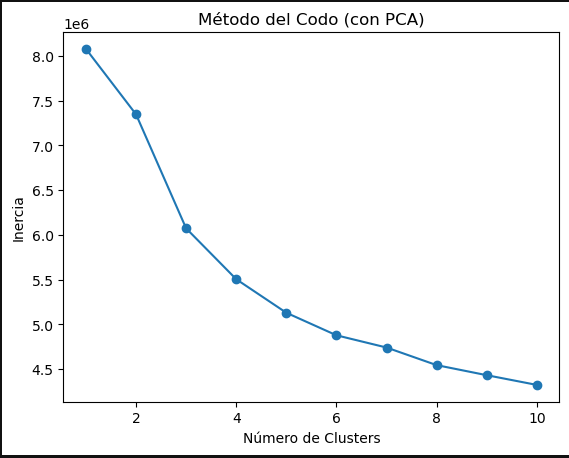
\includegraphics[width=0.60\textwidth]{4/figures/Modelo_4.png}
    \caption{Representación de la Inercia utilizando el método del codo.}
    \label{fig:convolucion}
\end{figure}


\subsection{Aplicación de K-means}

Una vez definido el número óptimo de clústeres, se aplica el algoritmo de K-means al conjunto de datos que contiene las características combinadas de Histogram of Oriented Gradients (HOG) y Convolutional Neural Networks (CNN). Este proceso permite agrupar los frames en categorías o clústeres específicos, basados en patrones de similitud en sus características visuales.

Para cada frame en el conjunto de datos, K-means asigna una etiqueta de clúster que indica a cuál grupo pertenece. Esta asignación se integra en el \texttt{DataFrame} original, permitiendo así un análisis estructurado de cada frame dentro de su grupo correspondiente.

\begin{figure}[H]
    \centering
    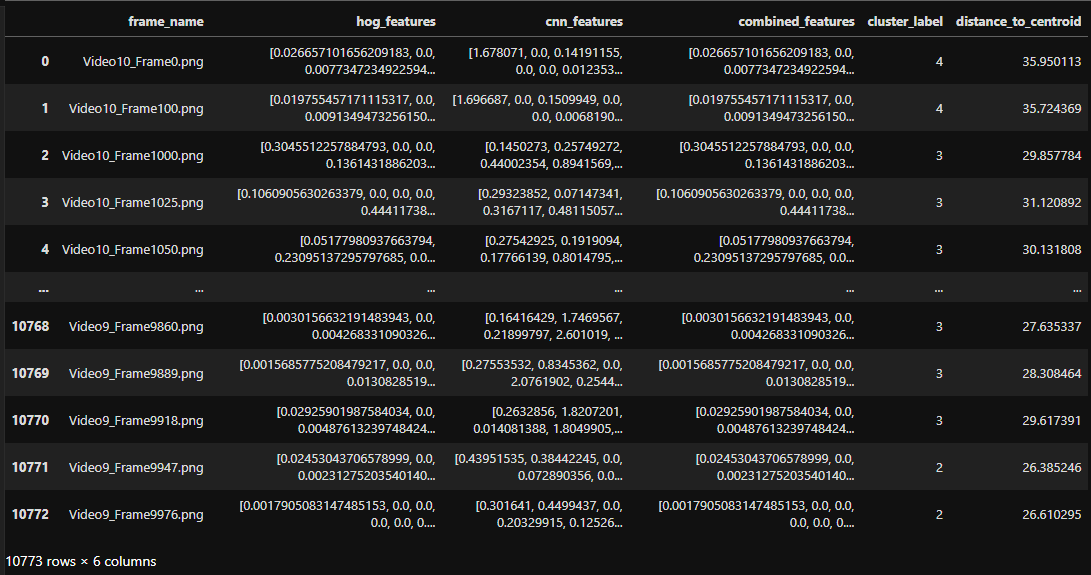
\includegraphics[width=0.80\textwidth]{4/figures/KNN_1.png}
    \caption{Asignación de clusters y distancias al centroide correspondiente.}
    \label{fig:convolucion}
\end{figure}

Además de la etiqueta de clúster, el algoritmo calcula la distancia de cada frame al centroide de su clúster. Esta distancia es fundamental para determinar el grado de representatividad de cada frame dentro de su grupo. Los frames más cercanos al centroide se consideran más representativos del clúster, mientras que aquellos a mayor distancia pueden representar características menos comunes. Esta información se incluye como una columna adicional en el \texttt{DataFrame} y es utilizada en análisis posteriores, como la selección de frames clave para la generación de clips representativos.


\subsection{Selección de frames clave}
Para cada cluster, identificamos los frames más representativos, es decir, aquellos más cercanos a los centroides, y los almacenamos en la lista \texttt{frames\_clave}.

Los frames seleccionados como representativos de cada cluster se muestran en una única imagen combinada. Esto proporciona una vista consolidada de los elementos clave de cada cluster.

\begin{figure}[H]
    \centering
    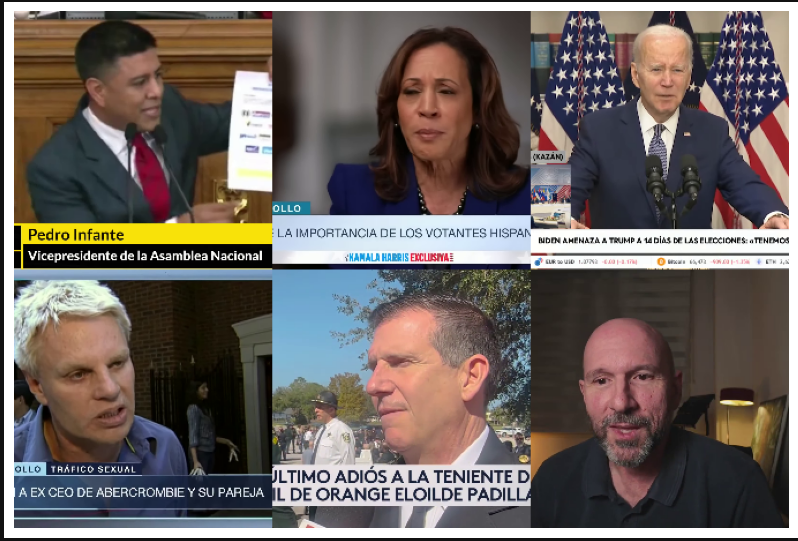
\includegraphics[width=0.60\textwidth]{4/figures/Frames_1.png}
    \caption{Características principales de la carpeta de frames generada.}
    \label{fig:convolucion}
\end{figure}

\section{Generación de Clips a partir de Frames Clave}

En esta sección se detalla el proceso de generación de clips de video basados en frames clave seleccionados en el análisis de clusters. Este proceso permite crear un video final que resalta los eventos representativos, proporcionando un contexto visual adicional para cada frame clave.

\subsection{Descripción del Proceso}
El proceso de generación de clips se lleva a cabo en tres etapas principales:

\begin{itemize}
    \item \textbf{Identificación de frame clave}: Cada frame clave se asocia con un video específico y se establece un rango de frames adyacentes a ese frame clave, seleccionado en base a la distancia temporal del evento destacado.
    \item \textbf{Selección de frames adyacentes}: Se seleccionan un conjunto de frames anteriores y posteriores al frame clave. Esto permite capturar el contexto visual necesario para proporcionar una vista completa del evento.
    \item \textbf{Combinación de clips}: Los clips individuales, correspondientes a cada frame clave y sus frames adyacentes, se concatenan en un solo video continuo que representa una síntesis de los eventos clave.
\end{itemize}

\subsection{Visualización de Resultados}
La Figura \ref{fig:clip_muestra} muestra el clip generado a partir de frames clave y sus frames adyacentes, destacando la coherencia visual que resulta de esta selección.

\begin{figure}[H]
    \centering
    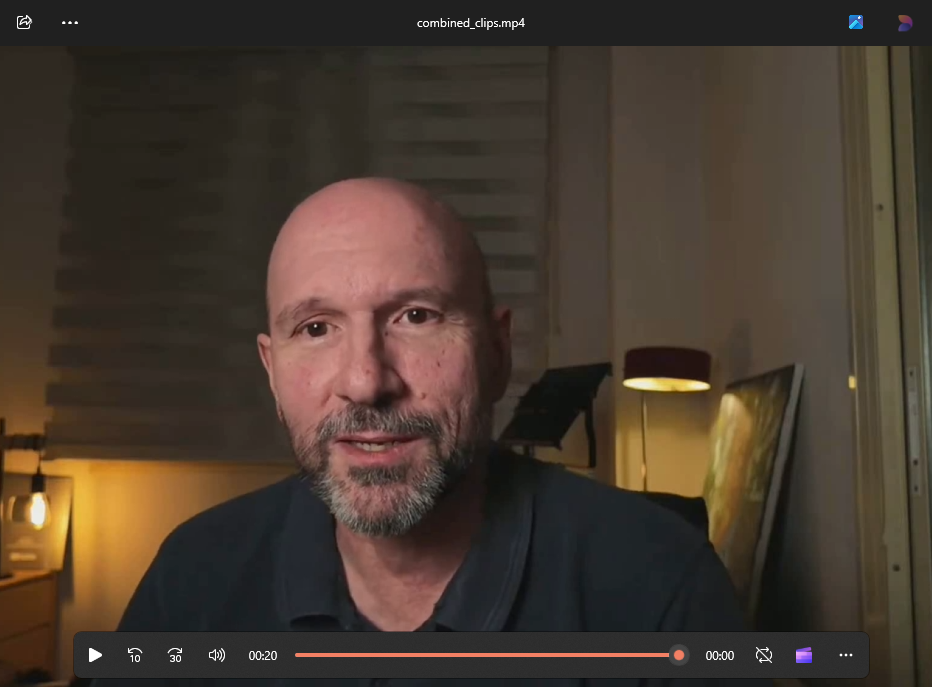
\includegraphics[width=0.8\textwidth]{4/figures/Clip_1.png}
    \caption{Muestra de frames clave y sus frames adyacentes.}
    \label{fig:clip_muestra}
\end{figure}

La Tabla \ref{tab:video_info} presenta un resumen de las especificaciones del video generado.

\begin{table}[H]
    \centering
    \caption{Especificaciones del Video Generado a partir de Frames Clave}
    \begin{tabular}{l c}
        \hline
        \textbf{Atributo} & \textbf{Valor} \\
        \hline
        Nombre del Video & combined\_clips.mp4 \\
        Resolución & 1920x1080 \\
        Duración (s) & 20.22 \\
        FPS & 29.97 \\
        \hline
    \end{tabular}
    \label{tab:video_info}
\end{table}


%\chapter{ANÁLISIS Y DISCUSIÓN DE RESULTADOS}
\section{X}

Hello, here is some text without a meaning.  This text should 
show what a printed text will look like at this place.  If you 
read this text, you will get no information.  Really?  Is there 
no information?  Is there a difference between this text and some 
nonsense like ``Huardest gefburn?  Kjift " not at all!...

\begin{table}
	\centering
	\begin{tabular}{l|r}
		Item & Quantity \\\hline
		Widgets & 42 \\
		Gadgets & 13
	\end{tabular}
	\caption{\label{tab:widgetxcxs}An example table.}
\end{table}

\section{Y}

Nisi porta lorem mollis aliquam ut porttitor leo. Aenean pharetra magna ac placerat vestibulum. Est placerat in egestas erat imperdiet sed euismod. Velit euismod in pellentesque massa placerat. Enim praesent elementum facilisis leo vel fringilla. Ante in nibh mauris cursus mattis molestie a iaculis. Erat pellentesque adipiscing commodo elit at imperdiet dui accumsan sit. Porttitor lacus luctus accumsan tortor posuere ac ut. Tortor at auctor urna nunc id. A iaculis at erat pellentesque adipiscing commodo elit. 


\section{Z}

Nisi porta lorem mollis aliquam ut porttitor leo. Aenean pharetra magna ac placerat vestibulum. Est placerat in egestas erat imperdiet sed euismod. Velit euismod in pellentesque massa placerat. Enim praesent elementum facilisis leo vel fringilla. Ante in nibh mauris cursus mattis molestie a iaculis. Erat pellentesque adipiscing commodo elit at imperdiet dui accumsan sit. Porttitor lacus luctus accumsan tortor posuere ac ut. Tortor at auctor urna nunc id. A iaculis at erat pellentesque adipiscing commodo elit.

%\chapter{CONCLUSIONES Y RECOMENDACIONES}
\section{Conclusiones}

Hello, here is some text without a meaning.  This text should 
show what a printed text will look like at this place.  If you 
read this text, you will get no information.  Really?  Is there 
no information?  Is there a difference between this text and some 
nonsense like ``Huardest gefburn?  Kjift " not at all!...



\section{Recomendaciones}

Nisi porta lorem mollis aliquam ut porttitor leo. Aenean pharetra magna ac placerat vestibulum. Est placerat in egestas erat imperdiet sed euismod. Velit euismod in pellentesque massa placerat. Enim praesent elementum facilisis leo vel fringilla. Ante in nibh mauris cursus mattis molestie a iaculis. Erat pellentesque adipiscing commodo elit at imperdiet dui accumsan sit. Porttitor lacus luctus accumsan tortor posuere ac ut. Tortor at auctor urna nunc id. A iaculis at erat pellentesque adipiscing commodo elit. 


\chapter{Anexo II: Resumen de Papers investigados}
%\section{Conclusiones}

\begin{table}[h]
	\newcommand{\multirot}[1]{\multirow{2}{*}[-8ex]{\rotcell{\rlap{#1}}}}
	%\scriptsize
	\footnotesize
	\centering
	\begin{tabular}{|m{0.5cm}|m{0.3cm}|m{4cm}|m{2cm}|m{0.6cm}|m{1.7cm}|m{3cm}|} 
		\hline
		\rowcolor[rgb]{0,0.251,0.502} \multicolumn{1}{|c|}{\textcolor{white}{Tipo}} & \multicolumn{1}{c|}{\textcolor{white}{N°}} & \multicolumn{1}{c|}{\textcolor{white}{Título}}                                                                             & \multicolumn{1}{c|}{\textcolor{white}{Autor}}        & \multicolumn{1}{c|}{\textcolor{white}{Año}} & \multicolumn{1}{c|}{\textcolor{white}{País}} & \multicolumn{1}{c|}{\textcolor{white}{Fuente}}                                                        \\ 
		\hline
		\multirot{Problema}                                        & 1                                             & DeepASL: Enabling Ubiquitous and Non-IntrusiveWord and
		Sentence-Level Sign Language Translation~                                                                               & Biyi Fang, Jillian Co, Mi Zhang                                 & 2018                                        & USA                               & Michigan State University                                                                                      \\ 
		\cline{2-7}
		& 2                                             & Sign Language Fingerspelling Recognition Using Depth
		Information and Deep Belief Networks                                                            & Hai-Feng Zhao                     & 2017                                        & China                                  & Huaiyin Institute of Technology                                                \\ 
		\hline
		\multirow{3}{*}[-14ex]{\rotcell{\rlap{Propuesta}}}
		& 3                                             & Deep learning-based sign language recognition system for static signs~                           & Ankita Wadhawan                             & 2019                                        & USA                                          & Neural Computing and Applications                                                                    \\ 
		\cline{2-7}
		& 4                                             & Enabling Real-time Sign Language Translation on Mobile Platforms
		with On-board Depth Cameras~                                                                                & HYEONJUNG PARK                                          & 2021                                        & Sout Korea                                          & School of Integrated Technology                                                             \\ 
		\cline{2-7}
		& 5                                             & Computational Model for Sign Language Recognition in a Colombian Context                                               & Nelson Ortiz-Farfán, Jorge E. Camargo-Mendoza & 2020                                        & Colombia                                          & 2016 IEEE/ACIS 15th International Conference on Computer and
		Information Science (ICIS)             \\ 
		\hline
		\multirow{4}{*}[-28ex]{\rotcell{\rlap{Técnica}}}                                          & 6                                             & Stock Prices Prediction using the Title of Newspaper Articles
		with Korean Natural Language Processing~                   & Yun, Sim,  Seok                                      & 2019                                        & Japan                                        & 2019 International Conference on Artificial Intelligence in
		Information and Communication (ICAIIC)  \\ 
		\cline{2-7}
		& 7                                             & A Method of Optimizing LDA Result Purity Based on Semantic
		Similarity                                                    & Jingrui, Z., Qinglin, W., Yu, L.,  Yuan, L.          & 2017                                        & China                                        & 2017 32nd Youth Academic Annual Conference of Chinese
		Association of Automation (YAC)~              \\ 
		\cline{2-7}
		& 8                                             & Qualitative Stock Market Predicting with Common Knowledge Based
		Nature Language Processing: A Unified View and Procedure & Rao, D., Deng, F., Jiang, Z.,  Zhao, G.~             & 2015                                        & USA                                          & 2015 7th International Conference on Intelligent Human-Machine
		Systems and Cybernetics              \\ 
		\cline{2-7}
		& 9                                             & Fuzzy Bag-of-Words Model for Document Representation                                                                       & Zhao, R.,  Mao, K.                                   & 2018                                        & USA                                          & IEEE Transactions on Fuzzy Systems (~Volume:
		26~,~Issue: 2~, April 2018~)                           \\
		\hline
	\end{tabular}
	\caption{Cuadro Resumen de Papers investigados. Fuente: Elaboración propia}
\label{A:table}
\end{table}

%% Anexos
\appendix
\renewcommand{\appendixname}{Anexos}
\renewcommand{\appendixtocname}{Anexos}
\renewcommand{\appendixpagename}{Anexos}
\clearpage
\addappheadtotoc
\appendixpage
\chapter{Anexo I: Matriz de Consistencia}

\begin{figure}[h]
	\begin{center}
		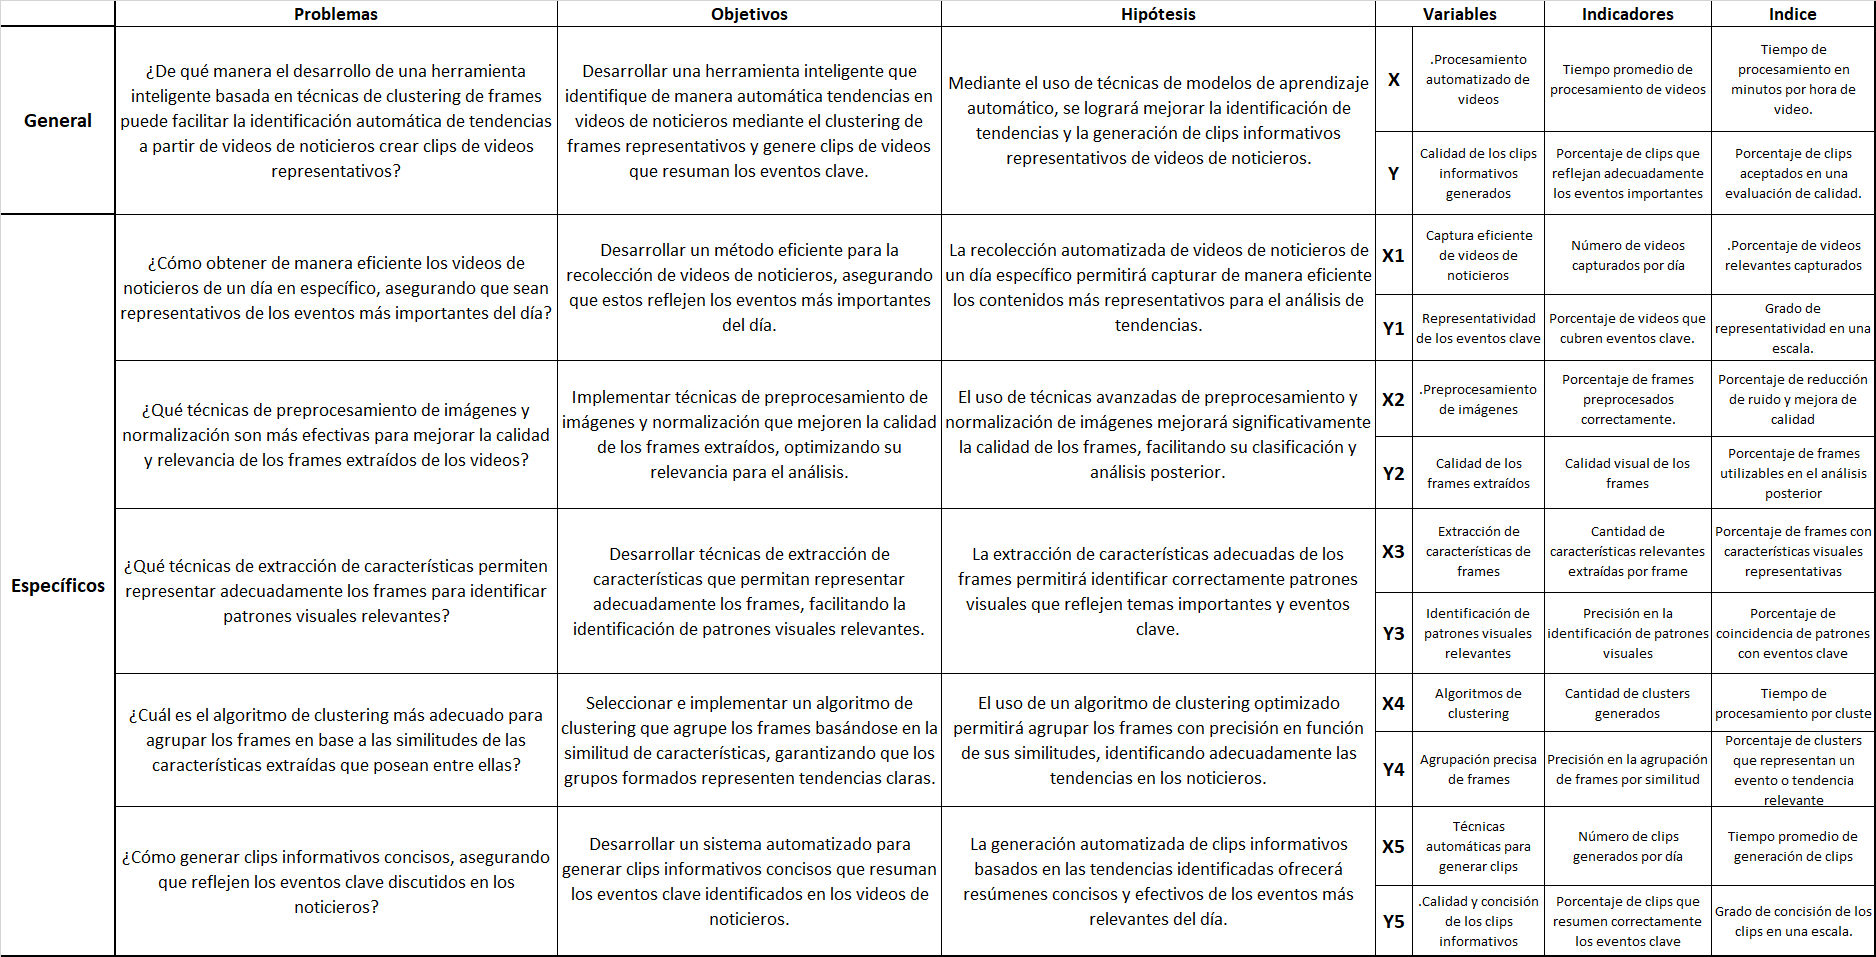
\includegraphics[angle=90, width=0.6\textwidth]{images_repo/matriz-consistecia.png}
		\caption{Matriz de consistencia Completo. Fuente: Elaboración propia}
		\label{1:fig 13}
	\end{center}
\end{figure}
\chapter{Anexo II: Árbol de problemas}
\begin{figure}[h]
	\begin{center}
		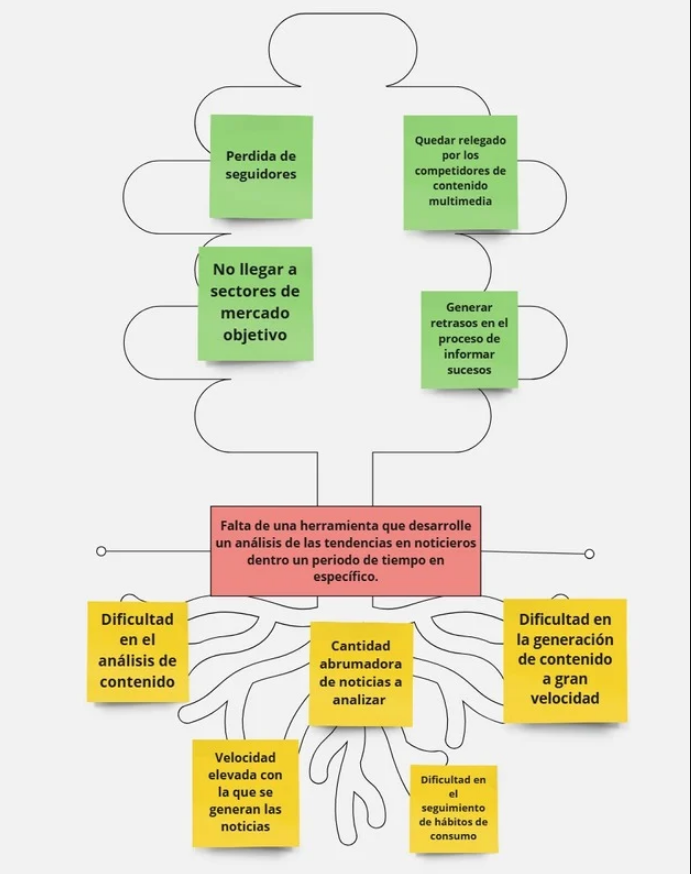
\includegraphics[width=0.7\textwidth]{images_repo/arbol_problemas.png}
		\caption{Árbol de problemas. Fuente: Elaboración propia}
		\label{1:fig 14}
	\end{center}
\end{figure}









%% Bibliografía
\printbibliography[heading=bibintoc,title={BIBLIOGRAFÍA}]

\end{document}
